\documentclass[MS]             % MS thesis dissertation.
              {iitmdiss_as}    % Hacked by hyperbolicme.
%              {iitmdiss}      % If the powers to be are finicky.

\usepackage{times}             % Font?
\usepackage{t1enc}             % T1 encoding??  
%\usepackage{boxedminipage}
\usepackage{../lib/mythesislib}
\usepackage{../lib/mylatexlib}
% \usepackage{comment}           % DEBUG ONLY

\def \mythesissubmissiondate {10 January 2012}
\def \mythesissubmissionmonth {\MakeUppercase {January 2012}}

\begin{document}
%%%%%%%%%%%%%%%%%%%%%%%%%%%%%%%%%%%%%%%%%%%%%%%%%%%%%%%%%%%%%%%%%%%%%%
% Title page
\title{\mythesistitleNOTSYNPOSIS} 
\author{\myname} 
\date{
  {\mythesissubmissionmonth}} 
\department{\MakeUppercase{\mythesisdept}}
%\department{\mythesisdept}

%\nocite{*}
\maketitle

%%%%%%%%%%%%%%%%%%%%%%%%%%%%%%%%%%%%%%%%%%%%%%%%%%%%%%%%%%%%%%%%%%%%%%
% Certificate
\certificate

\vspace*{0.5in}
  
\noindent 
This is to certify that the thesis titled {\bf \mythesistitleNOTSYNPOSIS},
submitted by {\bf \myname}, to the {\bf Indian Institute of Technology
Madras}, for the award of the degree of {\bf \mydegree}, is 
a bona fide record of the research work done by her under our
supervision.  The contents of this thesis, in full or in parts, have
not been submitted to any other Institute or University for the award
of any degree or diploma.

\vspace*{1.5in}

\begin{singlespacing}
  \hspace*{-0.25in}
  \parbox{3in}{
    \noindent {\bf Dr.~\myadvisor} \\
    \small
    \noindent Research Guide\\
    \noindent Associate Professor\\
    \noindent Dept. of \mydept\\
    \noindent IIT Madras -- 600 036
  } \hfill
  \parbox{1.25in}{               % {1.75in}
    \small
    \vspace*{0.75in}
    \begin{tabular}[h]{r}
    \noindent {Chennai}\\         
    \noindent {\mythesissubmissiondate} 
    \end{tabular}
  }
\end{singlespacing}


%%%%%%%%%%%%%%%%%%%%%%%%%%%%%%%%%%%%%%%%%%%%%%%%%%%%%%%%%%%%%%%%%%%%%%
% Acknowledgements
\acknowledgements

\tnote{WIP}

%%%%%%%%%%%%%%%%%%%%%%%%%%%%%%%%%%%%%%%%%%%%%%%%%%%%%%%%%%%%%%%%%%%%%%
% Abstract

\begin{abstract}
  \noindent {\em {\bf Keywords}: \hspace*{0.5em} \parbox[t]{4.4in}{consecutive
    ones property, algorithmic graph theory, hypergraph isomorphism,
    interval labeling}} \vspace*{24pt}

  \def \tem {}
  \noindent 
  Consecutive-ones property is a non-trivial property of binary
  matrices that has been studied widely in the literature for over
  past 50 years. Detection of COP in a matrix is possible efficiently
  and there are several algorithms that achieve the same. This thesis
  documents the work done on an extension of COP extended from the
  equivalent interval assignment problem in \cite{nsnrs09}. These new
  results rigorously prove a natural extension (to trees) of their
  characterization as well as makes connections to graph isomorphism,
  namely path graph isomorphism.

  \tnote{EXPAND. 
  Abstract must be a brief about what results we have and how it fits
  in the body of research.\\
  -- Area: Broad to Specialized. i.e. Combinatorial
    algorithms -> Matrix reorganization -> general data reorganization
    (interval assignment) -> path assignment\\
  -- Class of problems: say, data reorganization.\\
  -- Nature of results: Is a generalization. We have a
    Polynomial algorithm for a subset of the generalization.\\
% maybe add - we explore a natural
%     generalization of results on binary matrices with the |\tem
%     consecutive-ones property|.  We consider the following constraint
%     satisfaction problem. Given (i) a set system $\F \subseteq$
%     $(2^{U} \setminus \emptyset)$ of a finite set $U$ of cardinality
%     $n$, (ii) a tree $T$ of size $n$ and (iii) a bijection called
%     |\tem tree path labeling|, $\cl$ mapping the sets in $\cF$ to
%     paths in $T$, does there exist at least one bijection $\phi:U
%     \rightarrow V(T)$ such that for each $S \in \cF$, $\{\phi(x) \mid
%     x \in S\} = \cl(S)$?  A tree path labeling of a set system is
%     called |\tem feasible| if there exists such a bijection $\phi$.
%     We present an algorithmic characterization of feasible tree path
%     labeling. COP is a special instance of tree path labeling problem
%     when $T$ is a path.  We conclude with a polynomial time algorithm
%     to find a feasible tree path labeling of a given set system when
%     $T$ is a |\tem $k$-subdivided star|, set system has a single
%     containment tree of overlap components and set size is limited to
%     at most $k+2$.
  }
\end{abstract}

%\pagebreak

%%%%%%%%%%%%%%%%%%%%%%%%%%%%%%%%%%%%%%%%%%%%%%%%%%%%%%%%%%%%%%%%%
% Table of contents etc.

\begin{singlespace}
\tableofcontents
\thispagestyle{empty}

\listoftables
\addcontentsline{toc}{chapter}{LIST OF TABLES}
\listoffigures
\addcontentsline{toc}{chapter}{LIST OF FIGURES}
\end{singlespace}


%%%%%%%%%%%%%%%%%%%%%%%%%%%%%%%%%%%%%%%%%%%%%%%%%%%%%%%%%%%%%%%%%%%%%%
% Abbreviations
\abbreviations

\noindent 
\begin{tabbing}
xxxxxxxxxxx \= xxxxxxxxxxxxxxxxxxxxxxxxxxxxxxxxxxxxxxxxxxxxxxxx \kill
\textbf{COP}   \> Consecutive-ones Property \\
\textbf{COT}   \> Consecutive-ones Testing \\
\textbf{ICPIA}   \> Intersection Cardinality Preservation Interval Assignment \\
\textbf{ICPPL}   \> Intersection Cardinality Preserved Path Labeling \\
% ADD MORE HERE
\end{tabbing}

\pagebreak

%%%%%%%%%%%%%%%%%%%%%%%%%%%%%%%%%%%%%%%%%%%%%%%%%%%%%%%%%%%%%%%%%%%%%%
% Notation

\chapter*{\centerline{NOTATION}}
\addcontentsline{toc}{chapter}{NOTATION}

\begin{singlespace}
\begin{tabbing}
xxxxxxxxxxx \= xxxxxxxxxxxxxxxxxxxxxxxxxxxxxxxxxxxxxxxxxxxxxxxx \kill
\textbf{$2^{U}$}  \> Powerset of set $U$ \\
\end{tabbing}
\end{singlespace}

\pagebreak
\clearpage

% The main text will follow from this point so set the page numbering
% to arabic from here on.
\pagenumbering{arabic}

\chapter{Introduction}
\label{ch:intro}

Consecutive-ones property is a non-trivial property of binary matrices
that has been studied widely in the literature for over past 50
years. Detection of COP in a matrix is possible efficiently and there
are several algorithms that achieve the same. This thesis documents
the work done on an extension of COP extended from the equivalent
interval assignment problem in \cite{nsnrs09}. These new results
rigorously prove a natural extension (to trees) of their
characterization as well as makes connections to graph isomorphism,
namely path graph isomorphism.

\tnote{Have a para on Organization: Outline of document}
Section~\ref{sec:background} gives a brief survey of COP and
optimization problems related to it followed by motivation for the
thesis in Section~\ref{sec:motive}.  Section~\ref{sec:results}
presents a summary of our results on the extension of COP namely, the
tree path labeling problem. \tnote[TH]{update for thesis}


% \tnote{testing 1 2 3...}
% \tnote[bogus1]{testing 1 2 3...}
% \tnote[bogus2]{testing 1 2 3...}
% \tnote[GTC]{testing 1 2 3...}
% \tnote[bogus4]{testing 1 2 3...}
% \tnote[TH]{testing 1 2 3...}

\section{Illustration of the problem}
\label{sec:problem}

A group of students, \Pa, \Pig, \Sn, \Wo, \Vi, \Li, \Ch, \Sa, \Fr,
\Sc\ and \Lu\ enroll at the {\WSI} for a liberal arts programme.  As
part of their semester thesis, they pick a body of work to study and
form the namesake study groups, {\LLL}, {\GGG}, {\BBB} and
{\TTT}\tnote[TH]{put bib entries for these works!}. A student will be
in at least one study group and may be in more than one. For instance,
as will be seen later, {\Fr} studies both {\LLL} and {\TTT} while \Wo\
studies only \BBB.

Let $U$ and $\cF$ represent the set of students and the set of study
groups respectively and the integers $n$ and $m$ denote the total
number students and study groups respectively. In relation to this
example, these are defined in Table~\ref{tab:wsigroups}. Also given
there is the study group allocation to students.
 
\begin{table}[t]%[htbp]
  \centering
  { \footnotesize
  \begin{tabular}{rcl}
    $U $&$=$&$ \{\xPa,\; \xPi,\; \xSn,\; \xWo,\; \xVi,\; \xLi,\; \xCh,\;
    \xSa,\; \xFr,\; \xSc,\; \xLu\}$\\
    $\cF $&$=$&$ \{\xLLL, \xGGG, \xBBB, \xTTT\}$\\
    $\xLLL $&$=$&$ \{\xCh,\;  \xSa,\;  \xFr,\;  \xSc,\;  \xLu \}$\\
    $\xGGG $&$=$&$ \{\xPa,\;  \xPi,\;  \xVi,\;  \xCh \}$\\
    $\xBBB $&$=$&$ \{\xSn,\;  \xPi,\;  \xWo \}$\\
    $\xTTT $&$=$&$ \{\xVi,\;  \xLi,\;  \xCh,\;  \xFr \}$\\
    $n $&$=$&$ |U| = 11$\\
    $m $&$=$&$ |\cF| = 4$      
  \end{tabular}
}
  \caption{\figtabsize Students and study groups in \WSI}
  \label{tab:wsigroups}
\end{table}

The campus has a residential area {\residenceblock} that has $n$
single occupancy apartments reserved for the study groups'
accommodation.  All these apartments are located such that the streets
connecting them do {\em not} form
loops. Fig~\ref{fig:streetmappathpeople} \tnote[TH]{fig:streetmap}
shows the street map for {\residenceblock}. It may be noted that as a
graph, it classifies as a tree.


\begin{table}[htbp]
  \centering
  {\footnotesize    
    \begin{tabular}{l||l}
      \begin{tabular}{rcl}
        $T $&$=$&$ \text{\em Street map tree of \residenceblock}$\\
        $V(T) $&$=$&$ \{ 1, 2, 3, 4, 5, 6, 7, 8, 9, 10, 11 \}$\\
        $\cP $&$=$&$ \{R\xLLL, R\xGGG, R\xBBB, R\xTTT\}$\\
        $R\xLLL $&$=$&$ \{9, 1, 5, 3, 11\}$\\
        $R\xGGG $&$=$&$ \{7, 2, 6, 5\}$\\
        $R\xBBB $&$=$&$ \{8, 2, 4 \}$\\
        $R\xTTT $&$=$&$ \{10, 6, 5, 3\}$\\
        $n $&$=$&$ |V| = 11$\\
        $m $&$=$&$ |\cP| = 4$\\\\
        $\cl $&$=$& {\em Study group to route mapping}\\        
        $\cl(\mathbb{X}) $&$=$&  $R\mathbb{X}$ for all $\mathbb{X} \in
        \cF$
      \end{tabular} & 
      \begin{tabular}{c}
       {\em Apartment allocation }($\phi$)\\
                    \begin{tabular}{c|c}                      
                      1  & \xSa\\
                      2  & \xPi\\
                      3  & \xFr\\
                      4  & \xWo\\
                      5  & \xCh\\
                      6  & \xVi\\
                      7  & \xPa\\
                      8  & \xSn\\
                      9  & \xLu\\
                      10 & \xLi\\
                      11 & \xSc                     
                    \end{tabular}
      \end{tabular}\\
    \end{tabular}
  }
  \caption{\figtabsize A solution to study group accommodation problem}
  \label{tab:iltree}
\end{table}

A natural question would be to find how the students should be
allocated apartments such that each study group has the {\em least
  distance to travel} for a discussion? More specifically, we are
interested in enforcing additional conditions, namely, that all the
students in a study group must be next to each other; in other words,
for one student to reach another fellow study group member's apartment
(for all study groups the student is part of), she must not have to
pass the apartment of any student who is not in that study group. To
further elucidate, the apartments of students of any study group must
be arranged in an exclusive unfragmented path on the street
map. Exclusivity here means that the path must not have apartments
from other study groups (unless that apartment is also part of {\em
  this} study group).

An intuitive approach to this problem would be to first find the paths
that each study group decides to inhabit and then refine the
allocation to individual students. A feasible allocation of exclusive
routes to study groups is illustrated in
Fig~\ref{fig:streetmappathpeople} \tnote[TH]{fig:streetmappath} and
the students' allocation of apartments that obeys this route
allocation is also shown. Table~\ref{tab:iltree} shows the same
solution set theoretically.  How this is algorithmically computed is
the focus of this thesis.

\begin{figure}[htbp] %[t]%
 \centering
  (a) 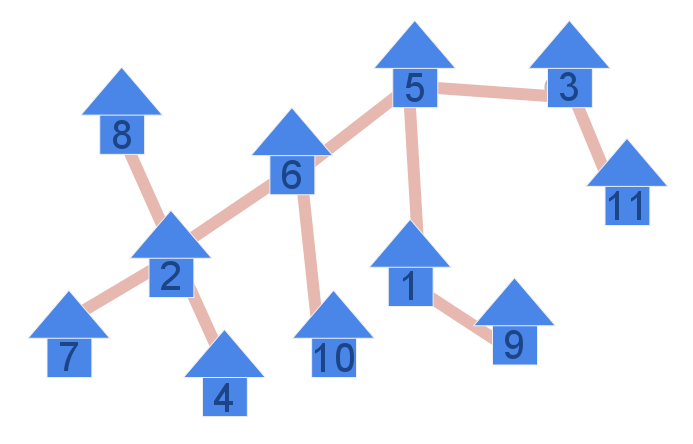
\includegraphics[scale=0.2]{../img/1_infinite_loop.png}
  (b) 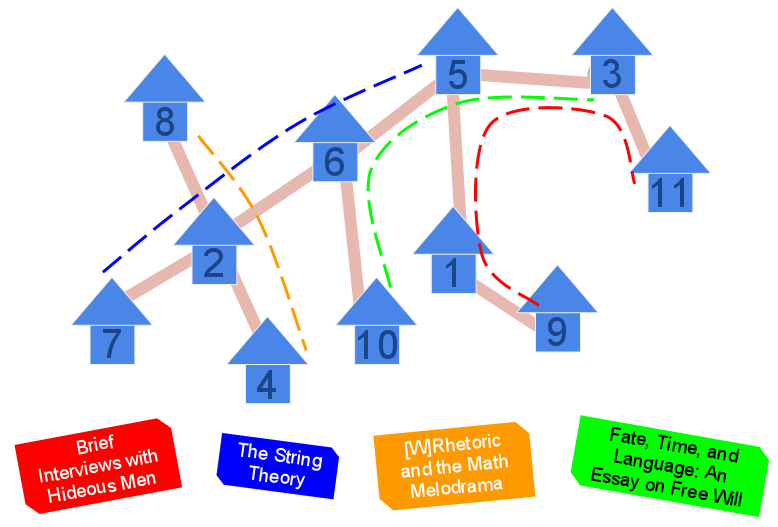
\includegraphics[scale=0.2]{../img/2_infinite_loop_BTWF.png}

 \label{fig:streetmap}
 \caption{\figtabsize (a) {\residenceblock} street map (b)
   {\residenceblock} street map with study group routes
   allocated. Routes are color coded as follows: red for
   \textcolor{red}{$\xLLL$} group, blue for \textcolor{blue}{$\xGGG$}
   group, orange for \textcolor{yellow}{$\xBBB$} group, green for
   \textcolor{green}{$\xTTT$} group}

 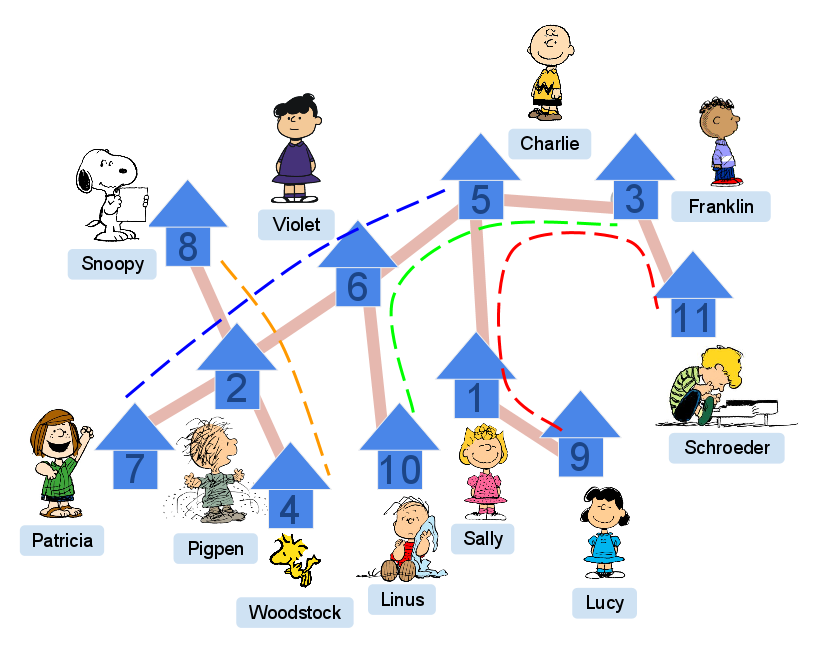
\includegraphics[scale=0.5]{../img/3_infinite_loop.png}
  \caption{\figtabsize Individual allocation of apartments to students
    in {\residenceblock} that meets the requirements stated before.
    The routes are color coded as follows: red for
    \textcolor{red}{$\xLLL$} group, blue for \textcolor{blue}{$\xGGG$}
    group, orange for \textcolor{yellow}{$\xBBB$} group, green
    for \textcolor{green}{$\xTTT$} group. {\tiny {\em Peanuts images
        {\copyright} Charles Schulz}}}% YellowOrange
  \label{fig:streetmappathpeople}
\end{figure}
\tnote{UPDATE IMAGE (b) 2-infinite-loop-BTWF.png. REMOVE TITLES. ADD
  {$\xLLL$} {$\xGGG$} {$\xBBB$} {$\xTTT$}}

\tnote[TH]{make dashed/textured lines for routes. make it color
  agnostic.}

As a special case, suppose all the apartments are on the same street
or if they are all lined up on a single path, the street map becomes a
tree that is just a path. Then the problem becomes what is called an
{\em interval assignment problem}. The idea of interval assignment may
not be obvious here; hence to see this, consider a different problem
in {\WSI} where the classes for these study groups courses need to be
scheduled during a day (or a week or any time period). Each study
group has a bunch of courses associated with it some of which may be
shared by two or more study groups. It is mandatory that a student who
is a member of a study group takes all the courses associated with
that group. There are slots during the day for classes to be held and
the problem is to allocate class slots to courses such that all the
classes of a study group are consecutive. It is debatable if this will
not hamper the attention span and memory retention rate of the
students but that is, regrettably, out of the scope of this
thesis. The parallels between this class allocation problem and the
accommodation problem can be seen as follows. The set $U$ here, are
the courses offered (say Course 101 {\coneohone}, Course 102
{\coneohtwo} and so on). In this variation of the problem, the
collection $\cF$ is the set of study groups but the study groups are
filled by course IDs (in place of students in the earlier
example). For instance, Course 101 is mandatory for all study groups
$\xLLL$, $\xGGG$, $\xBBB$, $\xTTT$ and Course 102 is mandatory for
only the $\xLLL$ group) and so on. The sequence of class slots for the
day (or week or any time period) is analogous to the street map in the
accommodation problem. It is quite obvious now why this version of the
problem (where the ``target graph'' is a path and not any
tree\tnote[TH]{Allowing any tree in this example could be seen as a
  scenario where there are parallel classes. A node falling in the
  path between two other nodes would mean that the corresponding is
  scheduled between the other two.}) is called an interval assignment
problem.

The interval assignment problem to a set system is equivalent to the
consecutive-ones property (COP) problem in binary matrices\cite{wlh02,
  nsnrs09}.  The COP problem is to rearrange rows (columns) of a
binary matrix in such a way that every column (row) has its {\un}s
occur consecutively. If this is possible the matrix is said to have
the COP.  COP is a well researched combinatorial problem and has
several positive results on tests for it and computing the COP
permutation (i.e. the course schedule in the above illustration) which
will be surveyed later in this document. Hence we are interested in
extensions of COP, more specifically, the extension of interval
assignment problem to tree path assignment problem (which is
illustrated by the study group accommodation problem).


\section{Basic preliminaries - general definitions and nomenclature}
\tnote{(definitions theorems etc) needed if any
    - graph theory}


\section{Consecutive-ones Property Testing - a Brief Survey}
\label{sec:background}

In this section, a brief survey of the consecutive-ones problem and its
optimization problems is presented.

%%%%%%                              %%%%%%
%THX is the second level of ``tnote''-ing%
%%%%%%                              %%%%%%
\tnote[TH]{ADD: As it will be described in detail later in this
  document, isomorphism of certain % classes of graphs, namely chordal
%   graphs, have a close relationship with consecutive-ones property and
%   generalizations of it.  This is perhaps because of how closely COP
%   of a matrix relates to properties of graphs derived from matrices as
%   seen in the following results.
}
\tnote[THX]{ADD: peo exists iff chordal. lexicographic BFS
  [tag:chordalGraph]} %
\tnote[THX]{ADD: A well known result in %perfect graph theory is that
%  the maximal cliques of  an interval graph $G$ can be linearly ordered
%   such that for all $v \in V(G)$, cliques containing $v$ are
%   consecutive in the ordering cite~{gh64}. This clearly means that a
%   graph $G$ is an interval graph if and only if
}% 
\tnote[THX]{verify
  from paper the statement of claim.}% 
\tnote[TH]{maximal clique vertex
  incidence matrix of%  $G$ has COP.  Also, maximal cliques of any
%   chordal graph can be enumerated in polytime $O(m+n)$
}
\tnote[THX]{citation?!!}%  
\tnote[TH]{cite~{fg65} uses these results to
  give the first polynomial time algorithm for COT.}%
\tnote[THX]{check. how do they use it?}%  
\tnote[TH]{ A bipartite graph
  is convex%  (on $R$) if and only if its half adjacency matrix has COP
%   on rows.  The results in cite~{bl76} on COT are based on the result
%   that interval graphs are AT-free chordal graphs.
}%
\tnote[THX]{the latter being Tucker's?}%  
\tnote[THX]{(2) TBD survey
  -- % see blue notes (in notebook) under Graph Isomorphism. namely
%   citations in cite:aas93 (3) a brief on heirarchy of chordal graphs,
%   path graphs, interval graphs, peo, clique tree etc. and results. (4)
%   interval graphs are incomparability graphs. see
%   Golumbic. [tag:classification] (5) finding min length hole in
%   bipartite graph is polynomial time [Sec 3.3.2 in cite:d08phd] (6)
%   theorem 2.2 in cite:d08phd - $G$ is union of v.d. caterpillars iff
%   $M$ has COP in rows. $M$ is edge vertex incidence matrix $(*,2)$ of
%   $G$
}%


\subsection{Matrices with COP}
\label{sec:copmatrices}
As seen earlier, the interval assignment problem (illustrated as the
course scheduling problem in Section~\ref{sec:problem}), is a special
case of the problem we address in this thesis, namely the tree path
labeling problem (illustrated as the study group accommodation
problem). The interval assignment problem and COP problem are equivalent
problems. In this section we will see some of the results that
exists in the literature today towards solving the COP problem and
optimization problems surrounding it.

\begin{figure}[t] %[htbp]
  \centering

  {\figtabsize
    \begin{tabular}[h]{l|lcccl}
      $M_1$: & $M_1'$: &&&& $M_2$:\\
      &&&&&\\
      \begin{tabular}[h]{llll}
        $c_1$ & $c_2$ &$c_3$ &$c_4$\\
        &&&\\
        \un & 0   & \un & 0\\
        0   & \un & 0   & \un \\
        \un & 0   & 0   & \un
      \end{tabular}
      &
      \begin{tabular}[h]{llll}
        $c_3$ &$c_1$ &$c_4$& $c_2$\\
        &&&\\
        \un & \un & 0 & 0\\
        0 & 0 & \un & \un \\
        0 & \un & \un & 0
      \end{tabular}
      &&&&
      \begin{tabular}[h]{llll}
        $d_1$ & $d_2$ &$d_3$ &$d_4$\\
        % &&&\\
        &&&\\
        \un & \un & 0 & 0\\
        0 & \un & \un & 0 \\
        0 & \un & 0 & \un 
      \end{tabular}
    \end{tabular}
  }

  \caption{\figtabsize Matrices with and without COP. $M_1$ has COP
    because by permuting its columns, $c_1$-$c_4$, one can obtain
    $M_1'$ where the {\un}s in each row are consecutive. $M_2$,
    however, does not have COP since no permutation of its columns,
    $d_1$-$d_4$, will arrange {\un}s in each row consecutively
    \cite{d08phd}.}

  \label{fig:cop-matrix}
\end{figure}

Recall that a matrix with COP is one whose rows (columns) can be
rearranged so that the {\un}s in every column (row) are in consecutive
rows (columns). Figure~\ref{fig:cop-matrix} shows examples of this
property.  COP in binary matrices has several practical applications
in diverse fields including scheduling \cite{hl06}, information
retrieval \cite{k77} and computational biology \cite{abh98}.  Further,
it is a tool in graph theory \cite{mcg04} for interval graph
recognition, characterization of Hamiltonian graphs, planarity testing
\cite{bl76} and in integer linear programming \cite{ht02,hl06}.


The obvious first questions after being introduced to the consecutive
ones property of binary matrices are if COP can be detected
efficiently in a binary matrix and if so, can the COP permutation of
the matrix also be computed efficiently?  Recognition of COP in a
binary matrix is polynomial time solvable and the first such algorithm
was given by \cite{fg65}.  A landmark result came a few years later
when \cite{at72} discovered the families of forbidden submatrices that
prevent a matrix from having COP and most, if not all, results that
came later were based on this discovery which connected COP in binary
matrices to convex bipartite graphs. In fact, the forbidden
submatrices came as a corollary to the discovery that convex bipartite
graphs are AT-free in \cite{at72}\tnote[TH]{check}. The first linear
time algorithm for COP testing (COT) was invented by \cite{bl76} using
a data structure called PQ trees.  Since then several COT algorithms
have been invented -- some of which involved variations of PQ trees
\cite{mm96,wlh01,mcc04}, some involved set theory and ICPIA
\cite{wlh02,nsnrs09}, parallel COT algorithms\cite{as95,bs03,ly91} and
certifying algorithms\cite{mcc04}. 

The construction of PQ trees in \cite{bl76} draws on the close
relationship of matrices with COP to interval graphs. A PQ tree of a
matrix is one that stores all row (column) permutations of the matrix
that give the COP orders (there could be multiple orders of rows or
columns) of the matrix. This is constructed using an elaborate linear
time procedure and is also a test for planarity\tnote[TH]{check check
  check. both interval graph and planarity in this paper?}.  PQR trees
is a generalized data structure based on PQ trees \cite{mm96,mpt98}.
\cite{tm05} describes an improved algorithm to build PQR
trees. \tnote[TH]{improv in terms of what?}\cite{wlh02} describes the
simpler algorithm for COT. Hsu also invented PC trees
\cite{wlh01}\tnote[TH]{This result first appeared inproc ISAAC92}
which is claimed to be much easier to implement. \cite{nsnrs09}
describes a characterization of consecutive-ones property solely based
on the cardinality properties of the set representations of the
columns (rows); every column (row) is equivalent to a set that has the
row (column) indices of the rows (columns) that have one entries in
this column (row). This is interesting and relevant, especially to
this thesis because it simplifies COT to a great degree. \tnote[TH]{it
  reduces the solution search space. fill in the blanks.}

\cite{mcc04} describes a different approach to COT. While all previous
COT algorithms gave the COP order if the matrix has the property but
exited stating negative if otherwise, this algorithm gives an evidence
by way of a certificate of matrix even when it has no COP. This
enables a user to verify the algorithm's result even when the answer
is negative. This is significant from an implementation perspective
because automated program verification is hard and manual verification
is more viable. Hence having a certificate reinforces an
implementation's credibility. Note that when the matrix {\em has} COP,
the COP order is the certificate.  The internal machinery of this
algorithm is related to the weighted betweenness problem
addressed\tnote[TH]{in what way??} in \cite{co98}.  \tnote[TH]{expand
  on the COP order graph creation and it having to be bipartite for M
  to have COP. and thus an odd cycle being an evidence of no COP.}
\tnote[TH]{ where should this go?: (1) cite|jlm97 (application of PQ trees
  in graphics). (2) helly's theorem citation
  19XXdgk-Hellystheorem-Danzer-Gruenbaum-Klee}


\subsection{Optimization problems in COP}
\label{sec:optcop}

So far we have been concerned about matrices that have the consecutive
ones property. However in real life applications, it is rare that data
sets represented by binary matrices have COP, primarily due to the
noisy nature of data available. At the same time, COP is not arbitrary
and is a desirable property in practical data representation
\cite{co98,jkckv04,k77}. In this context, there are several
interesting problems when a matrix does not have COP but is ``close''
to having COP or is allowed to be altered to have COP. These are the
optimization problems related to a matrix which does not have
COP. Some of the significant problems are surveyed in this section.

\tnote[TH]{ -- sect 4.1 in cite:d08phd has many results
  surveyed. hardness results, approx. results. results are usually for
  a class of matrices $(a,b)$ where number {\un}s in columns and rows
  are restriced to $a$ and $b$ . -- problem of flipping at most $k$
  entries of $M$ to make it attain COP. this is NP complete
  cite:b75-phd}\tnote[TH]{(1) scite:lb62 showed that interval graphs
  are AT-free.  describe AT (2) show the close relationship b/w COP
  and graphs sec 2.2, pg 31} \cite{at72} showed that a matrix that
does not have COP have certain substructures that prevent it from
having COP. Tucker classified these forbidden substructures into five
classes of submatrices. This result is presented in the context of
convex bipartite graphs which \cite{at72} proved to be
AT-free\tnote[TH]{ check this up. give details. - doms'}. By
definition, convex bipartite graph have half adjacency matrices that
have COP on either rows or columns (graph is biconvex if it has COP on
both)\cite{d08phd}. A half adjacency matrix is a binary matrix
representing a bipartite graph as follows. The set of rows and the set
of columns form the two partitions of the graph. Each row node is
adjacent to those nodes that represent the columns that have {\un}s in
the corresponding row. \cite{at72} proves that this bipartite graph
has no asteroidal triple if and only if the matrix has COP and goes on
to identify the forbidden substructures for these bipartite
graphs. The matrices corresponding to these substructures are the
forbidden submatrices.

Once a matrix has been detected to not have COP (using any of the COT
algorithms mentioned earlier), it is naturally of interest to find out
the smallest forbidden substructure (in terms of number of rows and/or
columns and/or number of entries that are {\un}s). \cite{d08phd}
discusses a couple of algorithms which are efficient if the number of
{\un}s in a row is small. This is of significance in the case of sparse
matrices where this number is much lesser than the number of
columns. $(*,\Delta)${\em -matrices} are matrices with no restriction
on number of {\un}s in any column but has at most $\Delta$ {\un}s in
any row. {\sc Min COS-R (Min COS-C), Max COS-R (Max COS-C)} are
similar problems which deals with inducing COP on a matrix. In {\sc
  Min COS-R (Min COS-C)} the question is to find the minimum number of
rows (columns) that must be deleted to result in a matrix with COP.
In the dual problem {\sc Max COS-R (Max COS-C)} the search is for the
maximum number of rows (columns) that induces a submatrix with
COP. Given a matrix $M$ with no COP, \cite{b75-phd} shows that finding
a submatrix $M'$ with all columns\tnote[TH]{check if b75 deals with
  COP col or COP row. also is it any submatrix with k less than r rows
  or submatrix must have all columns?} but a maximum cardinality
subset of rows such that $M'$ has COP is NP complete. \cite{hg02}
corrects an error of the abridged proof of this reduction as given in
\cite{gj79}.  \cite{d08phd} discusses all these problems in detail
giving an extensive survey of the previously existing results which
are almost exhaustively all approximation results and hardness
results. Taking this further, \cite{d08phd} presents new results in
the area of parameterized algorithms for this
problem\tnote[TH]{elaborate - what are the results?}.

Another problem is to find the minimum number of entries in the matrix
that can be toggled to result in a matrix with COP.  \cite{v85}
discusses approximation of {\sc COP Augmentation} which is the problem
of changing of the minimum number of zero entries to {\un}s so that
the resulting matrix has COP. As mentioned earlier, this problem is
known to be NP complete due to \cite{b75-phd}. \cite{v85} also proves,
using a reduction to the longest path problem, \tnote[TH]{or is it a
  survey of another result?  check.} that finding a Tucker's forbidden
submatrix of at least $k$ rows is NP complete. \tnote[TH]{how is this
  different from booth's 75 result??}  \tnote[TH]{where should this
  go? cite|tz04 (approx submatrix with COP sparse matrices)}

\cite{jkckv04} discusses the use of matrices with almost-COP (instead
of one block of consecutive {\un}s, they have $x$ blocks, or {\em
  runs}, of consecutive {\un}s and $x$ is not too large) in the
storage of very large databases.  The problem is that of reordering of
a binary matrix such that the resulting matrix has at most $k$ runs of
{\un}s. This is proved to be NP hard using a reduction from the
Hamiltonian path problem.\tnote[TH]{Theorem 2.1 in jkckv}
\tnote[TH]{(1) A connection of COP problem to the travelling salesman
  problem is also introduced. what does this mean? -- COP can be used
  as a tool to reorder $0.5T \le runs(M) \le T$. (2) The optimization
  version of the $k$-run problem, i.e. minimization of number of
  blocks of ones is proven to be NP complete by
  cite:k77}\tnote[TH]{are these two the same?} \tnote[TH]{what is the
  reduction?} \tnote[TH]{other problems similar to COP -- cite:ckl96
  (ILP, circ ones, one drop) -- cite:th98 (generalization of COP -
  minimax, biotonic column) Tucker}



\section{********* Application of COP in Areas of Graph Theory and
  Algorithms}
\label{sec:appcopGTA}

\subsection{********* COP in Relational Database Model}
\label{sec:apprdbm}
\tnote{(set systems theme)}

\subsection{********* COP in Graph Isomorphism}
\label{sec:appgraphiso}
\tnote{(canonization theme)}

\subsection{********* Certifying Algorithms}
\label{sec:appcertalgo}
\tnote{ (certification McC04 theme)}


\section{Generalization of COP - the Motivation}
\label{sec:motive}
Section~\ref{sec:copmatrices} introduced a succinct characterization
for consecutive-ones property which is solely based on the cardinality
properties of the set representations of the matrix's columns
\cite{nsnrs09}. This result is very relevant to this thesis because
aside from it simplifying COT to a great degree, our generalization
problem is motivated by their results.

\cite{nsnrs09} characterizes interval assignments to the sets which
can be obtained from a single permutation of the rows.  For an
assignment to be feasible, the cardinality of the interval assigned to
each set in the system must be same as the cardinality of the set, and
the intersection cardinality of any two intervals must be same as the
intersection cardinality of their corresponding sets.  While this is
obviously a necessary condition, this result shows this is also
sufficient.  \cite{nsnrs09} calls this an Intersection Cardinality
Preserving Interval Assignment (ICPIA).  This paper generalizes the
idea from \cite{wlh02} of decomposing a given binary matrix into prime
matrices for COT and describes an algorithm to test if an ICPIA exists
for a given set system.

The equivalence of the problem of testing for the consecutive-ones
property to the constraint statisfaction problem of interval
assignment \cite{nsnrs09} or interval labeling \cite{kklv10} is as
follows. Every column (row) of the binary matrix can be converted into
a set of non-negative integers which are the indices of rows (columns)
with {\un}s in that column (row). It is apparent that if the matrix
has COP in columns (rows), then constructing such sets after applying
the COP permutation to the rows (columns) of the matrix will result in
sets with consecutive integers. In other words, after application of
COP reordering, the sets are intervals. Indeed the problem now becomes
finding interval assignments to a given set system such that there
exists a permutation of the universe of set of row indices (column
indices) which converts each set to its assigned interval.

The problem of interest in this thesis, namely, tree path labeling
problem, is a natural generalization of the interval assignment
problem or the COT problem. The problem is defined as follows -- given
a set system $\cF$ from a universe $U$ and a target tree $T$, does
there exist a bijection from $U$ to the vertices of $T$ such that each
set in the system maps to a path in $T$.  We refer to this as the
{\CFTPL} problem or simply {\em tree path labeling} problem for an
input set system and target tree pair -- $(\cF,T)$. The special case
of the target tree being a path, is the interval assignment problem.
We focus on generalizing the notion of an ICPIA \cite{nsnrs09} to
characterize feasible path assignments.  We show that for a given set
system $\cF$, a tree $T$, and an assignment of paths from $T$ to the
sets, there is a feasible\footnote{The notion of {\em feasibility} is
  formally defined in Section~\ref{ch:prelims}.}  bijection between
$U$ and $V(T)$ if and only if the intersection cardinalities among any
three sets (not necessarily distinct) is equal to that of the
corresponding paths assigned to them and the input passes a filtering
algorithm (described in this paper) successfully.  This algorithmic
characterization gives a natural data structure that stores all the
\remove{relevant} feasible bijections between $U$ and $V(T)$. This
reduces the search space for the solution considerably from the
universe of all possible bijections between $U$ and $V(T)$ to only
those bijections that maintain the characterization.  Further, the
filtering algorithm is also an efficient algorithm to test if a tree
path labeling\footnote{The terms {\em tree path labeling} and {\em
    tree path assignment} are, in informal language,
  synonyms. Formally, the former refers to the bijection $\cl: \cF
  \rightarrow \cP$. The latter refers to the set of ordered pairs
  $\{(S, P) \mid S \in \cF, P \in \cP\}$. $\cP$ is a set of paths on
  $T$.} is feasible.


\section{Summary of New Results in this Thesis}
\label{sec:results}

We see in Section~\ref{sec:motive} that pairwise intersection
cardinality preservation is necessary and sufficient for an interval
assignment to be feasible for a given hypergraph\footnote{A {\em
    hypergraph} is an alternate representation of a set system and
  will be used in this thesis. See Section~\ref{ch:prelims} for the
  formal definition.} and thus is a characterization for COP
\cite{nsnrs09}. \tnote{Refer to the survey section that will list the
  theorems and/or lemma?} In our work we extend this characterization
and find that trio-wise intersection cardinality preservation makes a
tree path labeling \footnote{A {\em tree path labeling} $\cl$ is a
  bijection of paths from the target tree $T$ to the hyperedges in
  given hypergraph $\cF$.  See Section~\ref{ch:prelims} for the formal
  definition.}  (TPL) feasible, which is a generalization of the COP
problem. This problem is defined as follows.

{\small
  \begin{minipage}[h]{5in}
    % \begin{singlespace}
    \vspace{2mm}
    {\large \FTPL}\\
    \begin{tabular}[t]{l|l}
      \hline\\
      {\tt Input} & 
      \begin{minipage}[t]{\probdefwidth}
        A hypergraph $\cF$ with vertex set $U$, a tree $T$, a set of
        paths $\cP$ from $T$ and a
        bijection $\cl$~$:$~$\cF \rightarrow \cP$.\\
      \end{minipage}\\
      {\tt Question} &
      \begin{minipage}[t]{\probdefwidth}
        Does there exist a bijection $\phi$~$:$~$U \rightarrow V(T)$
        such that $\phi$ when applied on any hyperedge in $\cF$ will
        give
        the path mapped to it by the given tree path labeling $\cl$.\\
        { i.e., $\cl(S) = \{\phi(x) \mid x \in S\}$, for every
          hyperedge $S \in \cF$.}
      \end{minipage}\\
    \end{tabular}
    % \end{singlespace}
  \end{minipage}\\
}

We give a necessary and sufficient condition by way of {\em
  Intersection Cardinality Preservation Path Labeling} (ICPPL) and a
filtering algorithm for {\FTPL} to output in affirmative. ICPPL
captures the trio-wise cardinality property described
earlier\footnote{See Section~\ref{sec:feasible} for the definition of
  ICPPL.}. This characterization can be checked in polynomial time.  A
relevant consequence of this constructive procedure is that it is
sufficient to iteratively check if three-way intersection
cardinalities are preserved.  In other words, in each iteration, it is
sufficient to check if the intersection of any three hyperedges is of
the same cardinality as the intersection of the corresponding paths.
Thus this generalizes the well studied question of the feasible
interval assignment problem which is the special case when the target
tree $T$ is simply a path \cite{wlh02,nsnrs09}.

Aside from checking if a given TPL is feasible, we also solve the
problem of computing a feasible TPL for a given hypergraph and target
tree, if one exists. This problem, {\CFTPL}, is defined as follows.

{\small
  \begin{minipage}[h]{5in}
    % \begin{singlespace}
    \vspace{2mm}
    {\large \CFTPL}\\
    \begin{tabular}[t]{l|l}
      \hline\\
      {\tt Input} & 
      \begin{minipage}[t]{\probdefwidth}
        A hypergraph $\cF$ with vertex set $U$ and a tree $T$.\\
      \end{minipage}\\

      {\tt Question} &
      \begin{minipage}[t]{\probdefwidth}
        Does there exist a set of paths $\cP$ from $T$ and a bijection
        $\cl$~$:$~$\cF \rightarrow \cP$, such that {\FTPL} returns
        {\bf true} on $(\cF, T, \cl)$.
      \end{minipage}\\
    \end{tabular}
    % \end{singlespace}
  \end{minipage}\\
}

We present a polynomial time algorithm for {\CFTPL} when the target
tree $T$ belongs to a special class of trees called {\em \kstar s} and
when the hyperedges in the hypergraph $\cF$ have at most $k+2$
vertices. A couple of examples of {\kstar s} are given in
Figure~\ref{fig:ksubstar}.

\begin{figure}[t]
  \centering
  \begin{tabular}[h]{ccccc}
    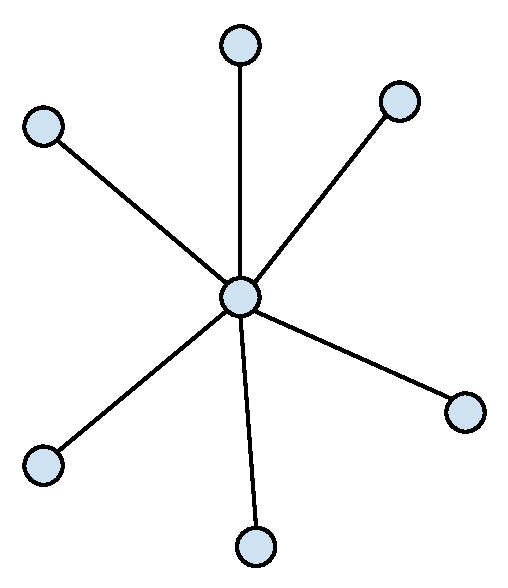
\includegraphics[scale=0.3]{../img/star.pdf} &&&&
    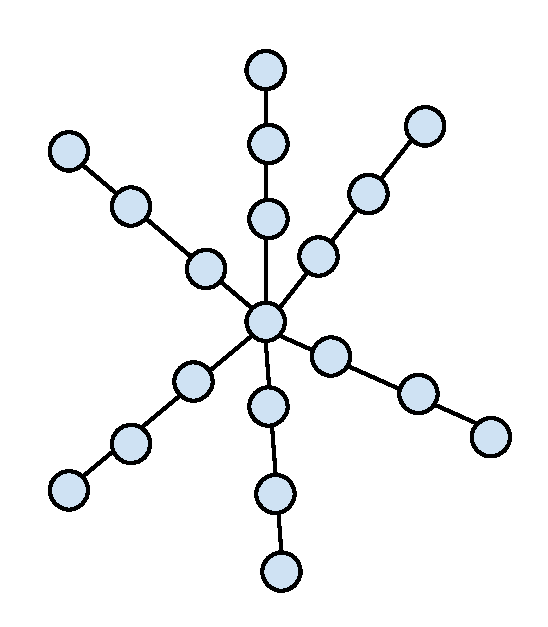
\includegraphics[scale=0.3]{../img/kstar.pdf}\\
    (a) &&&& (b)
  \end{tabular}
  \caption{\figtabsize Examples of {\kstar s}. (a) $k = 0$ (b) $k = 2$
  }
  \label{fig:ksubstar}
\end{figure}

{\small
  \begin{minipage}[h]{5in}
    % \begin{singlespace}
    \vspace{2mm}
    {\large \CFTPLKTREE}\\
    \begin{tabular}[t]{l|l}
      \hline\\
      {\tt Input} & 
      \begin{minipage}[t]{\probdefwidth}
        A hypergraph $\cF$ with vertex set $U$ such that every
        hyperedge
        $S \in \cF$ is of cardinality at most $k+2$ and a {\kstar} $T$.\\
      \end{minipage}\\
      {\tt Question} &
      \begin{minipage}[t]{\probdefwidth}
        Does there exist a set of paths $\cP$ from $T$ and a bijection
        $\cl$~$:$~$\cF \rightarrow \cP$, such that {\FTPL} returns
        {\bf true} on $(\cF, T, \cl)$.
      \end{minipage}\\
    \end{tabular}
    % \end{singlespace}
  \end{minipage}\\
}

\tnote{The following sentence seems out of place in this para} In
spite of this being a restricted case, we believe that our results are
of significant interest in understanding the nature of {\sc Graph
  Isomorphism} which is polynomial time solvable in interval graphs
while being hard on path graphs\cite{kklv10}. {\kstar s} are a class
of trees which are in many ways very close to intervals or paths. Each
ray\footnote{The path from a leaf to the root, the vertex with highest
  degree, is called a {\em ray} of the \kstar. See
  Section~\ref{ch:prelims}.} are independent except for the
root\footnote{The vertex with maximum degree in a {\kstar} is called
  {\em root}. See Section~\ref{ch:prelims}.} and hence can be
considered as an independent interval till the root. Our algorithm
builds on this fact and uses the interval assignment
algorithm\cite{nsnrs09} up until ``reaching'' the root and then uses
the trio-wise intersection cardinality (the extra condition in ICPPL
that generalizes ICPIA) check to resolve the ambiguity about which ray
the algorithm should ``grow'' the solution into in the next iteration.

We also have an algorithm for solving {\CFTPL} with no restrictions on
the target tree or set size which runs in exponential time.  This
algorithm finds a path labeling from $T$ by decomposing the problem
into subproblems of finding path labeling of subsets of $\cF$ from
subtrees of $T$. Given the fact that binary matrices naturally
represent a set system (see Section~\ref{sec:motive}) and that the
{\em overlap}\footnote{}\tnote{Give informal definition of ``overlap''
  in footnote and link to sec:prelims. ADD the definition in prelim.}
relation between the sets involved is an obvious equivalence relation,
$\cF$ quite naturally partitions into equivalence classes known as
{\em overlap components}\tnote{Give informal definition of ``overlap
  components'' in footnote and link to sec:prelims. ADD the definition
  in prelim.}. In the context of COP, overlap components were used in
\cite{wlh02} and \cite{kklv10}. Moreover, \cite{nsnrs09} discovered
that these equivalence classes form a total order \tnote{Give informal
  definition of ``total order'' in footnote?}. We extend this to TPL
and find that when $\cF$ is a path hypergraph\footnote{If there exists
  an FTPL for a hypergraph $\cF$, it is called a path hypergraph.},
the classes can be partially ordered as an in-tree in polynomial
time. Once $\cF$ is ``broken'' into overlap components, one must
identify the subtree of $T$ that it needs to map to and this is the
hard part which is currently open to be solved in polynomial time.

\tnote[TH]{The connection of TPL to graph isomorphism will be made
  later in the document}

\chapter{Consecutive-ones Property - a Survey of Important Results}
\label{ch:copsurvey}
\tnote{TBD: have a few lines about organization of chapter}

\tnote{ Survey chapter: is the full fledged expansion of the survey in
  introduction with details, observations, theorems etc.}

\section{Matrices with COP}
\label{sec:surveycoptest}
\tnote{Expand on ref:sec:copmatrices}

\section{Optimization problems in COP}
\label{sec:surveycopopt}
\tnote{Expand on ref:sec:optcop}


\section{********* COP in Relational Database Model}
\label{sec:surveyrdbm}
\tnote{Expand on sec:apprdbm}
\tnote{(set systems theme)}

\subsection{********* COP in Graph Isomorphism}
\label{sec:surveygraphiso}
\tnote{Expand on sec:appgraphiso}
\tnote{(canonization theme)}

\subsection{********* Certifying Algorithms}
\label{sec:surveycertalgo}
\tnote{Expand on sec:appcertalgo}
\tnote{ (certification McC04 theme)}


\chapter{Tree Path Labeling of Path Hypergraphs - the New Results}
\label{ch:myresearch}

\tnote{UPDATE TO FINAL VERSION. BELOW IS OLDER VERSION WITH INCOMPLETE
  SEC 4.}  This chapter documents all the new results obtained by us in the
area of tree path labeling of path hypergraphs which is the parent
problem addressed in this thesis. In Section~\ref{sec:motive} we see
that consecutive-ones property and its equivalent problem of interval
labeling of a hypergraph is a special case of the general problem of tree
path labeling of path hypergraphs.


\tnote{UPDATE the following para to current skeleton.}The necessary
preliminaries with definitions etc. are presented in
Section~\ref{ch:prelims}. Section~\ref{sec:feasible} documents the
characterization of a feasible path labeling for any path labeling
from any target trees. Section~\ref{sec:spltargettree} describes the
special case where the target tree is of a particular family of trees
and specifically, Section~\ref{sec:ksubdivstar} describes a polynomial
time algorithm to find the tree path labeling of a given set system
from a given $k$-subdivided tree. Section~\ref{sec:norestraint}
describes the general situation where the target tree has no
restrictions and the algorithm to find a TPL, if any, in this case.


\section{Introduction} 

The problem of consecutive-ones property testing can be easily seen as
a simple constraint satisfaction problem involving a hypergraph or a
system of sets from a universe. Every column (row) of the binary
matrix can be converted into a set of non-negative integers which are
the indices of the rows (columns) with {\un}s in that column
(row). When observed in this context, if the matrix has the COP on
columns (rows), a reordering of its rows (columns) will result in sets
that have only consecutive integers. In other words, the sets after
applying the COP row (column) permutation are intervals.  In this
form, one can see that this is indeed the problem of finding interval
assignments to the given set system \cite{nsnrs09} with a single
permutation of the universe (set of row or column indices for COP of
columns or rows, respectively) which permutes each set to its
interval. The result in \cite{nsnrs09} characterizes interval
assignments to the sets which can be obtained from a single
permutation of the rows (columns). They show that for each set, the
cardinality of the interval assigned to it must be same as the
cardinality of the set, and the intersection cardinality of any two
sets must be same as the intersection cardinality of the corresponding
intervals. This is a necessary and sufficient
condition. \tnote{(ICPIA) put reference to survey chapter}.  Finally,
the idea of decomposing a given binary matrix into prime matrices to
check for COP is adopted from cite|wlh02| to test if an ICPIA exists
for a given set system.\tnote{REPEATITION from intro chapter. but idea
  recall is necessary. so keep it but reword it to avoid monotone.}

A natural generalization of the interval assignment problem is
feasible tree path labeling problem of a set system. The problem is
defined as follows -- given a set system $\cF$ from a universe $U$ and
a tree $T$, does there exist a bijection from $U$ to the vertices of
$T$ such that each set in the system maps to a path in $T$.  We refer
to this as the {\em tree path labeling problem} for an input set
system, target tree pair -- $(\cF,T)$. \tnote{USE THE FORMAL PROBLEM DEF BLOCK}
%\begin{tabular}[t]{c}
{\small
\begin{minipage}[h]{5in}
 % \begin{singlespace}
 \vspace{2mm}
 {\large \FTPL}\\
 \begin{tabular}[t]{l|l}
 \hline\\
    {\tt Input} & 
    \begin{minipage}[t]{\probdefwidth}
      A hypergraph $\cF$ with vertex set $U$, a tree $T$, a set of
      paths $\cP$ from $T$ and a
      bijection $\cl$~$:$~$\cF \rightarrow \cP$.\\
    \end{minipage}\\
    {\tt Question} &
    \begin{minipage}[t]{\probdefwidth}
      Does there exist a bijection $\phi$~$:$~$U \rightarrow V(T)$
      such that $\phi$ when applied on any hyperedge in $\cF$ will
      give
      the path mapped to it by the given tree path labeling $\cl$.\\
      { i.e., $\cl(S) = \{\phi(x) \mid x \in S\}$, for every hyperedge
        $S \in \cF$.}
    \end{minipage}\\
  \end{tabular}
  % \end{singlespace}
\end{minipage}\\
}
%\end{tabular}



As a special case if the tree
$T$ is a path, the problem becomes the interval assignment problem. \tnote{USE THE FORMAL PROBLEM DEF BLOCK}
We focus on the question of generalizing the notion of an ICPIA
\cite{nsnrs09} to characterize feasible path assignments.  We show
that for a given set system $\cF$, a tree $T$, and an assignment of
paths from $T$ to the sets, there is a feasible bijection between $U$
and $V(T)$ if and only if all intersection cardinalities among any
three sets (not necessarily distinct) is same as the intersection
cardinality of the paths assigned to them and the input runs a
filtering algorithm (described in this paper) successfully.  This
characterization is proved constructively and it gives a natural data
structure that stores all the relevant feasible bijections between $U$
and $V(T)$.  Further, the filtering algorithm is also an efficient
algorithm to test if a tree path labeling to the set system is
feasible.  This generalizes the result in \cite{nsnrs09}.

In the later part of this paper, we focus on a new special case of the
tree path labeling problem. Here the set system is such that every set
is at most $k+2$ in size and for every pair of sets in it there exists
a sequence of sets between them with consecutive sets in this sequence
having a strict intersection -- i.e., non-empty intersection with
neither being contained in the other. Moreover, the given tree is a
{\em $k$-subdivided star}. We demonstrate a polynomial time algorithm
to find a feasible path labeling in this case.


\section{Preliminaries to new results}
\label{ch:prelims} 

\tnote{TBD: have a few lines about organization of chapter}This
section states definitions and basic facts necessary in the scope of
this document.

\tnote{Move some of this to general prelim in chapter 1}

The set $\F \subseteq (2^{U} \setminus \emptyset)$ is a {\em set
  system} of a universe $U$ with $|U| = n$.  The {\em support} of a
set system $\F$ denoted by $supp(\cF)$ is the union of all the sets in
$\F$; $supp(\F) = \bigcup_{S \in \F}S$. For the purposes of this
paper, a set system is required to ``cover'' the universe; $
supp(\cF) = U$.

The graph $T$ represents a {\em target tree} with same
number of vertices as elements in $U$; $|V(T)| = n$.  A {\em path
  system}\, $\cP$ is a set system of paths from $T$; $\cP \subseteq \{P
\mid P \subseteq V, \text{ } T[P] \text{ is a path} \}$.

% 
% A set system $\cF$ can be alternatively represented by a {\em
%   hypergraph} $\H_\cF$ whose vertex set is $supp(\cF)$ and
% hyperedges are the sets in $\cF$. This is a known representation for
% interval systems in literature \cite{bls99,kklv10}.  We extend this
% definition here to path systems.

A set system $\cF$ can be alternatively represented by a {\em
  hypergraph}\, $\cF_H$ whose vertex set is $supp(\cF)$ and hyperedges
are the sets in $\cF$. This is a known representation for interval
systems in literature \cite{bls99,kklv10}.  We extend this definition
here to path systems. Due to the equivalence of set system and
hypergraph in the scope of this paper, we drop the subscript $_H$ in
the notation and refer to both the structures by $\cF$.

Two hypergraphs $\cF'$, $\cF''$ are said to be {\em isomorphic} to
each other, denoted by $\cF' \cong \cF''$, iff there exists a
bijection $\phi: supp(\cF') \rightarrow supp(\cF'')$ such that for all
sets $A \subseteq supp(\cF')$, $A$ is a hyperedge in $\cF'$ iff $B$ is
a hyperedge in $\cF''$ where $B = \{\phi(x) \mid x \in A\}$
\cite{kklv10}. This is called {\em hypergraph
  isomorphism}. \tnote{also extend $\phi$ to hyperedges -- see if
  required }

The {\em intersection graph}\, $\bI(\cF)$ of a hypergraph $\cF$ is a
graph such that its vertex set has a bijection to $\cF$ and there
exists an edge between two vertices iff their corresponding hyperedges
have a non-empty intersection \cite{mcg04}.

If the intersection graphs of two hypergraphs are isomorphic,
$\bI(\cF) \cong \bI(\cP)$ where $\cP$ is also a path system, then the
bijection $\cl: \cF \rightarrow \cP$ due to this isomorphism is called
a {\em path labeling} of the hypergraph $\cF$. To illustrate further,
let $\cg: V(\cF) \rightarrow V(\cP)$ be the above mentioned
isomorphism where $V(\cF)$ and $V(\cP)$ are the vertex sets that
represent the hyperedges for each hypergraph respectively, $V(\cF) =
\{ v_S \mid S \in \cF\}$ and $V(\cP) = \{ v_P \mid P \in \cP\}$. Then
the path labeling $\cl$ is defined as follows: $\cl(S_1) = P_1$ iff
$\cg (v_{S_1}) = v_{P_1}$. The path system $\cP$ may be alternatively
denoted in terms of $\cF$ and $\cl$ as $\cF^\cl$. In most scenarios in
this paper, what is given are the pair $(\cF, \cl)$ and the target
tree $T$; hence this notation will be used more often.

If $\cF \cong \cP$ where $\cP$ is a path system, then $\cF$
is called a {\em path hypergraph} and $\cP$ is called {\em path
  representation} of $\cF$. If this isomorphism is $\phi: supp(\cF)
\rightarrow V(T)$, then it is clear that there is an {\em induced path
labeling} $\cl_\phi: \cF \rightarrow \cP$ to the set system;
$\cl_\phi(S) = \set{y \mid y = \phi(x), x \in S}$ for all $S \in \cF$. Recall that
$supp(\cP) = V(T)$.


A path labeling $(\cF, \cl)$ is defined to be {\em
  feasible} if
$\cF \cong \cF^\cl$ and this hypergraph isomorphism $\phi: supp(\cF)
\rightarrow supp(\cF^\cl)$ induces a path labeling $\cl_\phi: \cF
\rightarrow \cF^\cl$ such that $\cl_\phi = \cl$. 

An {\em overlap graph}\, $\bO(\cF)$ of a hypergraph $\cF$ is
a graph such that its vertex set has a bijection to $\cF$ and there
exists an edge between two of its vertices iff their corresponding
hyperedges overlap. Two hyperedges $S$ and $S'$ are said to {\em
  overlap}, denoted by $S \overlap S'$, if they have a non-empty
intersection and neither is contained in the other; $S \overlap S'
\text{ iff } S \cap S' \ne \emptyset, S \nsubseteq S', S' \nsubseteq
S$. Thus $\bO(\cF)$ is a spanning subgraph of $\bI(\cF)$ and not
necessarily connected. Each connected component of $\bO(\cF)$ is
called an {\em overlap component}.


A hyperedge $S \in \cF$ is called {\em marginal} if for all $S'
\overlap S$, the overlaps $S \cap S'$ form a single inclusion chain
\cite{kklv10}. Additionally, if $S$ is such that it is contained in no
other hyperedge in $\cF$, i.e., it is inclusion maximal then it is called
{\em super-marginal}.

A {\em star} graph is a complete bipartite graph $K_{1,p}$
which is clearly a tree and $p$ is the number of leaves. The vertex
with maximum degree is called the {\em center} of the star and the
edges are called {\em rays} of the star. A {\em $k$-subdivided star}
is a star with all its rays subdivided exactly $k$ times. The
definition of a {\em ray of a $k$-subdivided star} is extended to the path
from the center to a leaf. It is clear that all rays are of length $k+2$.




\section{Characterization of Feasible Tree Path  Labeling} 
\label{sec:feasible} 

In this section we give an algorithmic characterization of a
feasibility of tree path labeling.  Consider a path labeling $(\cF,
\cl)$ on the given tree $T$. We call $(\cF, \cl)$ an {\em Intersection
  Cardinality Preserving Path Labeling (ICPPL)} if it has the
following properties.

\begin{enumerate}[{(\icpplpr\ }i) \ \ \ ]
\item \label{pr:i} $|S| = |\cl(S)|$ \ \ \ \ \ \ \ \ \ \ \ \ \ \ \ \ \
  \ \ \ \ \ \ \ \ \ \ \ \ \ \ \ \ \ \ \ \ \ \ for all $S \in \cF$
  % \vspace{\topshrink}
\item \label{pr:ii}$|S_1 \cap S_2| = |\cl(S_1) \cap \cl(S_2)|$ \ \ \ \
  \ \ \ \ \ \ \ \ \ \ \ \ \ \ \ \ for all distinct $S_1, S_2 \in \cF$
  % \vspace{\topshrink}
\item \label{pr:iii}$|S_1 \cap S_2 \cap S_3| = |\cl(S_1) \cap \cl(S_2)
  \cap \cl(S_3)|$ \ \ \ for all distinct $S_1, S_2, S_3 \in \cF$
\end{enumerate}


The following lemma is useful in subsequent arguments. 
\begin{lemma}
  \label{lem:setminuscard}
  If $\cl$ is an ICPPL, and $S_1, S_2, S_3 \in \cF$, then $|S_1 \cap
  (S_2 \setminus S_3)| = |\cl(S_1) \cap (\cl(S_2) \setminus
  \cl(S_3))|$.
\end{lemma}
\begin{proof}%[Proof of Lemma~\ref{lem:setminuscard}]
  Let $P_i = \cl(S_i)$, for all $1 \le i \le  3$.
  $|S_1 \cap (S_2 \setminus S_3)| = |(S_1 \cap S_2) \setminus S_3| =
  |S_1 \cap S_2| - |S_1 \cap S_2 \cap S_3|$. Due to properties (ii)
  and (iii) of ICPPL, $|S_1 \cap S_2| - |S_1 \cap S_2 \cap S_3| = |P_1
  \cap P_2| - |P_1 \cap P_2 \cap P_3| = |(P_1 \cap P_2) \setminus P_3|
  = |P_1 \cap (P_2 \setminus P_3)|$. Thus lemma is proven. \qed
\end{proof}


In the remaining part of this section we show that $(\cF,
\cl)$ is feasible if and only if it is an ICPPL and
Algorithm~\ref{al:icppl-find-isomorph} returns a non-empty
function. Algorithm~\ref{al:icppl-find-isomorph} recursively does two levels of
filtering of $(\cF, \cl)$ to make it simpler while retaining the set
of isomorphisms, if any, between $\cF$ and $\cF^\cl$.
% One direction of this claim isclear: that if a path
% labeling is feasible, then all intersection cardinalities are
% preserved, i.e. the path labeling is an ICPPL. Algorithm~\ref{perms}
% \annote{has no premature exit condition hence any input will go
%   through it}{Prove that the filtered sets has ICPPL iff input PL
%   has ICPPL?}. Algorithm~\ref{leafasgn} has an exit condition at
% line~\ref{xempty}. It can be easily verified that $X$ cannot be
% empty if $\cl$ is a feasible path labeling. The reason is that a
% feasible path labeling has an associated bijection between
% $supp(\cF)$ and $V(T)$ \remove{i.e. $supp(\cF^{\cl})$} such that
% the sets map to paths, ``preserving'' the path labeling.  The rest
% of the section is devoted to constructively proving that it is
% sufficient for a path labeling to be an ICPPL and pass the two
% filtering algorithms.  To describe in brief, the constructive
% approaches refine an ICPPL iteratively, such that at the end of each
% iteration we have a ``filtered'' path labeling, and finally we have
% a path labeling that defines a family of bijections from $supp(\cF)$
% to $V(T)$\remove{ i.e. $supp(\cF^{\cl})$}.
First, we present Algorithm~\ref{perms} or {\tt filter\_1}, and prove
its correctness.  This algorithm refines the path labeling by
processing pairs of paths in $\cF^\cl$ that share a leaf until no two
paths in the new path labeling share any leaf.

\begin{algorithm}[h]
  \caption{Refine ICPPL {\tt filter\_1($\cF, \cl, T$)}}
  \label{perms}
  \begin{algorithmic}[\lndisplay]
    \STATE $\cF_0 \assign \cF$, $\cl_0(S) \assign \cl(S)$ for all $S \in \cF_0$\\
    \STATE $j \assign 1$\\
    \WHILE {there is $S_1, S_2 \in \cF_{j-1}$ such that
      $\cl_{j-1}(S_1)$ and $\cl_{j-1}(S_2)$ have a common leaf in
      $T$}\label{shareleaf} \STATE $\cF_j \assign (\cF_{j-1} \setminus
    \{S_1, S_2\})
    \cup \{S_1 \cap S_2, S_1 \setminus S_2, S_2 \setminus S_1 \}$ \label{setbreak} 
    \COMMENT {Remove $S_1$, $S_2$ and add the ``filtered'' sets}
    \STATE {\bf for} every $S \in \cF_{j-1}$ s.t. $S \ne S_1$ and $S \ne
    S_2$ {\bf do} $\cl_j(S) \assign \cl_{j-1}(S)$ {\bf end for}\\

    \STATE $\cl_j(S_1 \cap S_2) \assign \cl_{j-1}(S_1) \cap
    \cl_{j-1}(S_2)$
    \COMMENT {Carry forward the path labeling for all existing sets other than
      $S_1$, $S_2$}
    \STATE $\cl_j(S_1 \setminus S_2) \assign \cl_{j-1}(S_1) \setminus
    \cl_{j-1}(S_2)$ 
    \COMMENT {Define path labeling for new sets}
    \STATE $\cl_j(S_2 \setminus S_1) \assign \cl_{j-1}(S_2) \setminus
    \cl_{j-1}(S_1)$

    \IF{$(\cF_j, \cl_j)$ does not satisfy (\icpplpr~\ref{pr:iii}) of ICPPL}
    \label{ln:3waycheck}
    \STATE {\bf exit} \label{ln:exit1} \\
    \ENDIF

    \STATE $j \assign j+1$\\
    \ENDWHILE
    \STATE $\cF' \assign \cF_j$, $\cl' \assign \cl_j$\\
    \RETURN $(\cF', \cl')$
  \end{algorithmic}
\end{algorithm}

\begin{lemma} 
 \label{lem:feasible} 
 In Algorithm~\ref{perms}, if input $(\cF, \cl)$ is a feasible path
 assignment then at the end of $j$th iteration of the {\bf while}
 loop, $j \ge 0$, $(\cF_j, \cl_j)$ is a feasible path assignment.
\end{lemma}
\begin{proof}%[Proof of Lemma~\ref{lem:feasible}]
  We will prove this by mathematical induction on the number of
  iterations. The base case $(\cF_0, \cl_0)$ is feasible since it is
  the input itself which is given to be feasible. Assume the lemma is
  true till $j-1$th iteration. i.e. every hypergraph isomorphism
  $\phi: supp\left(\cF_{j-1}\right) \rightarrow V\left(T \right)$ that
  defines $(\cF, \cl)$'s feasibility, is such that the induced path
  labeling on $\cF_{j-1}$, $\cl_{\phi[{\cF_{j-1}}]}$ is equal to
  $\cl_{j-1}$. We will prove that $\phi$ is also the bijection that
  makes $(\cF_j, \cl_j)$ feasible. Note that $supp(\cF_{j-1}) =
  supp(\cF_{j})$ since the new sets in $\cF_j$ are created from basic
  set operations to the sets in $\cF_{j-1}$. For the same reason and
  $\phi$ being a bijection, it is clear that when applying the $\phi$
  induced path labeling on $\cF_j$, $ \cl_{\phi[{\cF_{j}}]}(S_1
  \setminus S_2) = \cl_{\phi[{\cF_{j-1}}]}(S_1) \setminus
  \cl_{\phi[{\cF_{j-1}}]}(S_2)$. Now observe that $ \cl_j(S_1
  \setminus S_2) = \cl_{j-1}(S_1) \setminus \cl_{j-1}(S_2) =
  \cl_{\phi[{\cF_{j-1}}]}(S_1) \setminus
  \cl_{\phi[{\cF_{j-1}}]}(S_2)$. Thus the induced path labeling
  $\cl_{\phi[{\cF_{j}}]} = \cl_{j}$. Therefore lemma is proven.  \qed
\end{proof}

\begin{lemma}
  \label{lem:invar1} In Algorithm~\ref{perms}, at the end of $j$th
  iteration, $j \ge 0$, of the {\bf while} loop, the following
  invariants are maintained.
  \begin{enumerate}[I {\ }] %\vspace{\topshrink}
  \item $\cl_j(R)$ is a path in $T$, \ \ \ \ \ \ \ \ \ \ \ \ \ \ \ \ \
    \ \ \ \ \ \ \ \ \ \ for all $R \in \cF_j$%\vspace{\topshrink}
  \item $|R| = |\cl_j(R)|$, \ \ \ \ \ \ \ \ \ \ \ \ \ \ \ \ \ \ \ \ \
    \ \ \ \ \ \ \ \ \ \ \ \ \ \ \ for all $R \in
    \cF_j$%\vspace{\topshrink}
  \item $|R \cap R'| = |\cl_j(R) \cap \cl_j(R')|$, \ \ \ \ \ \ \ \ \ \
    \ \ \ \ \ \ \ \ \ \ for all $R, R' \in \cF_j$%\vspace{\topshrink}
  \item $|R \cap R' \cap R''|=|\cl_j(R) \cap \cl_j(R') \cap
    \cl_j(R'')|$, \ \ \ for all $R, R', R'' \in \cF_j$
  \end{enumerate}
\end{lemma}

\begin{proof}
 Proof is by induction on the number of iterations, $j$. In this
  proof, the term ``new sets'' will refer to the sets added to $\cF_j$
  in $j$th iteration in line~\ref{setbreak} of Algorithm~\ref{perms},
  $S_1 \cap S_2, S_1 \setminus S_2, S_2 \setminus S_1$ and its
  images in $\cl_j$ where $\cl_{j-1}(S_1)$
  and $\cl_{j-1}(S_2)$ intersect and share a leaf.\\
  The invariants are true in the base case $(\cF_0, \cl_0)$, since it
  is the input ICPPL.  Assume the lemma is true till the $j-1$th
  iteration. Let us consider the possible cases for each of the above invariants for
  the $j$th iteration.

  
 \begin{enumerate}[\xbullet]
  \item {\em Invariant} I/II
    \begin{enumerate}[{I/II}a $|$] % \textbullet 
    \item {\em $R$ is not a new set.} It is in $\cF_{j-1}$. Thus
      trivially true by induction hypothesis.
    \item {\em $R$ is a new set.} If $R$ is in $\cF_{j}$ and not in
      $\cF_{j-1}$, then it must be one of the new sets added in
      $\cF_j$. In this case, it is clear that for each new set, the
      image under $\cl_j$ is a path since by definition the chosen
      sets $S_1$, $S_2$ are from $\cF_{j-1}$ and due to the while loop
      condition, $\cl_{j-1}(S_1)$, $\cl_{j-1}(S_2)$ have a
      common leaf. Thus invariant I is proven.\\
      Moreover, due to induction hypothesis of invariant III and the
      definition of $l_j$ in terms of $l_{j-1}$, invariant II is
      indeed true in the $j$th iteration for any of the new sets.  If
      $R = S_1 \cap S_2$, $|R| = |S_1 \cap S_2| = |\cl_{j-1}(S_1) \cap
      \cl_{j-1}(S_2)| = |\cl_j(S_1 \cap S_2)| = |\cl_j(R)|$.
      If $R = S_1 \setminus S_2$, $|R| = |S_1 \setminus S_2| = |S_1| -
      |S_1 \cap S_2| = |\cl_{j-1}(S_1)| - |\cl_{j-1}(S_1) \cap
      \cl_{j-1}(S_2)| = |\cl_{j-1}(S_1) \setminus \cl_{j-1}(S_2)| =
      |\cl_j(S_1 \setminus S_2)|
      = |\cl_j(R)|$. Similarly if $R = S_2 \setminus S_1$.\\
    \end{enumerate}
  \item {\em Invariant} III
    \begin{enumerate}[{III}a $|$]
    \item {\em $R$ and $R'$ are not new sets.} It is in
      $\cF_{j-1}$. Thus trivially true by induction hypothesis.
    \item {\em Only one, say $R$, is a new set.} Due to invariant IV
      induction hypothesis, Lemma~\ref{lem:setminuscard} and
      definition of $\cl_j$, it follows that invariant III is true no
      matter which of the new sets $R$ is equal to. If $R = S_1 \cap
      S_2$, $|R \cap R'| = |S_1 \cap S_2 \cap R'| = |\cl_{j-1}(S_1)
      \cap \cl_{j-1}(S_2) \cap \cl_{j-1}(R')| = |\cl_j(S_1 \cap S_2)
      \cap \cl_j(R')| = |\cl_j(R) \cap \cl_j(R')|$.  If $R = S_1
      \setminus S_2$, $|R \cap R'| = |(S_1 \setminus S_2) \cap R'| =
      |(\cl_{j-1}(S_1) \setminus \cl_{j-1}(S_2)) \cap \cl_{j-1}(R')| =
      |\cl_{j}(S_1 \cap S_2) \cap \cl_{j}(R')| = |\cl_{j}(R) \cap
      \cl_{j}(R')|$. Similarly, if $R = S_2 \setminus
      S_1$. Note $R'$ is not a new set.\\

    \item {\em $R$ and $R'$ are new sets.} By definition, the new
      sets and their path images in path label $\cl_j$ are disjoint so
      $|R \cap R'| = |\cl_j(R) \cap \cl_j(R)| = 0$. Thus case proven.
    \end{enumerate}
  \item {\em Invariant} IV
    
    Due to the condition in line~\ref{ln:3waycheck}, this invariant is
    ensured at the end of every iteration.
%     \begin{enumerate} [{Case 3.}1:]
%     \item {\em $R$, $R'$ and $R''$ are not new sets.} Trivially
%       true by induction hypothesis.
%     \item {\em Only one, say $R$, is a new set.}
%       If $R = S_1 \cap S_2$,  from Lemma~\ref{lem:fourpaths} and
%       invariant III hypothesis,  this case is proven. Similarly if $R$
%       is any of the other new  sets, the case is proven by also using
%       Lemma ~\ref{lem:setminuscard}.
%     \item {\em At least two of $R, R', R''$ are new sets.}
%       The new sets are disjoint hence this case is vacuously true.
%     \end{enumerate}
  \end{enumerate} \qed
%\vspace{-6mm} 

\end{proof}

\begin{lemma}
  \label{lem:noexit1}
  If the input ICPPL $(\cF, \cl)$ to Algorithm~\ref{perms} is
  feasible, then the set of hypergraph isomorphism functions that
  defines $(\cF, \cl)$'s feasibility is the same as the set that
  defines $(\cF_j, \cl_j)$'s feasibility, if any.  Secondly, for any
  iteration $j > 0$ of the {\em \bf while} loop, the {\em \bf exit}
  statement in line~\ref{ln:exit1} will not execute.
\end{lemma}
\begin{proof}
  Since $(\cF,\cl)$ is feasible, by Lemma~\ref{lem:feasible}
  $(\cF_j,\cl_j)$ for every iteration $j > 0$ is feasible.  % Therefore,
%   every hypergraph isomorphism $\phi: supp(\cF) \rightarrow V(T)$ that
%   induces $\cl$ on $\cF$ also induces $\cl_{j-1}$ and $\cl_{j}$ on
%   $\cF_{j-1}$ and $\cF_{j}$ respectively, i.e., $\cl_{\phi[\cF_{j-1}]}
%   = \cl_{j-1}$ and $\cl_{\phi[\cF_j]} = \cl_j$. Thus it can be seen
%   that for all $x \in supp(\cF)$, for all $v \in V(T)$ the following
%   hold true.
  Also, every hypergraph isomorphism $\phi: supp(\cF) \rightarrow
  V(T)$ that induces $\cl$ on $\cF$ also induces $\cl_{j}$ on
  $\cF_{j}$, i.e., $\cl_{\phi[\cF_j]} = \cl_j$. Thus it can be seen
  that for all $x \in supp(\cF)$, for all $v \in V(T)$, if $(x,v) \in
  \phi$ then $v \in \cl_{j}(S)$ for all $S \in \cF_{j}$ such that $x
  \in S$.
% the following
%   hold true.
%   \begin{enumerate}[i. ]
%   \item If $(x,v) \in \phi$ then $v \in \cl_{j-1}(S)$ for all $S \in
%     \cF_{j-1}$ such that $x \in S$.
%   \item If $(x,v) \in \phi$ then $v \in \cl_{j}(S)$ for all $S \in
%     \cF_{j}$ such that $x \in S$
%   \end{enumerate}
  In other words, filter 1 outputs a filtered path labeling that
  ``preserves''
  hypergraph isomorphisms of the original path labeling.\\
  Secondly, line~\ref{ln:exit1} will execute iff the exit condition in
  line~\ref{ln:3waycheck}, i.e. failure of three way intersection
  preservation, becomes true in any iteration of the {\em \bf while}
  loop.  Due to Lemma~\ref{lem:invar1} Invariant IV, the exit
  condition does not occur if the input is a feasible ICPPL.\qed

%   such that $\phi(x) = v$ where $v$ is the leaf considered in the
%   first iterations of while. Clearly, $\phi$ is a renaming of
%   vertices in hypergraph $\cF$ to those in hypergraph $\cF^\cl$. Thus
%   the following facts can be observed in every iteration of the loop.

%   \begin{enumerate}[\hspace{2mm}i. ] \vspace{\topshrink}
%   \item all intersection cardinalities are preserved in this path
%     labeling \vspace{\topshrink}
%   \item element $x$ is exclusive in a hyperedge in $\cF$ since $v$ is
%     exclusive in a hyperedge in $\cF^\cl$.
%   \end{enumerate}

%   Thus the exit condition is never rendered true after $x$ and $v$ are
%   removed from their respective hyperedges. \qed

% \noindent
% This proof uses mathematical induction on the number
%   of iterations $j$, $j \ge 0$, of the loop that executed
%   without exiting. The base case, $j = 0$ is obviously true since the
%   input is an ICPPL and the exit condition cannot hold true due to
%   ICPPL property (iii).  Assume the algorithm executes till the end
%   of $j-1$th iteration without exiting at line
%  ~\ref{ln:3waycheck}. Consider the $j$th iteration. From Lemma
%  ~\ref{lem:feasible} we know that $(\cF_j, \cl_j)$ and $(\cF_{j-1},
%   \cl_{j-1})$ are feasible\remove[AS]{and from the proof in lemma
%     lem:invar1 we know that $(\cF_{j-1}, \cl_{j-1})$ satisfies all the
%     invariants defined in the lemma}.  Thus there exists a bijection
%   $\phi: supp(\cF) \rightarrow V(T)$ such that the induced path
%   % labeling on $\cF_{j-1}$ $\cl_{\phi[\cF_{j-1}]} = \cl_{j-1}$.
%   labeling on $\cF_{j}$, $\cl_{\phi[\cF_{j}]}$ and on $\cF_{j-1}$,
%   $\cl_{\phi[\cF_{j-1}]}$ are equal to $\cl_{j}$ and $\cl_{j-1}$
%   respectively.  We need to prove that for any $R, R', R'' \in
%   \cF_{j}$, $|R \cap R' \cap R''| = |\cl_j(R) \cap \cl_j(R') \cap
%   \cl_j(R'')|$.
%   The following are the possible cases that could arise. From argument
%   above, $|\cl_j(R) \cap \cl_j(R') \cap \cl_j(R'')| =
%   |\cl_{\phi[\cF_{j}]}(R) \cap \cl_{\phi[\cF_{j}]} (R') \cap
%   \cl_{\phi[\cF_{j}]} (R'')|$

%   \begin{enumerate}[a $|$]
%   \item {\em None of the sets are new. $R, R', R'' \in \cF_{j-1}$.}
%     We know $(\cF_{j-1}, \cl_{j-1})$ is feasible. Thus $|R \cap R'
%     \cap R''| = |\cl_{j-1}(R) \cap \cl_{j-1}(R') \cap \cl_{j-1}(R'')|
%     = |\cl_{j}(R) \cap \cl_{j}(R') \cap \cl_{j}(R'')|$.
%   \item {\em Only one, say $R$, is a new set.}  Let $R = S_1 \cap S_2$
%     ($S_1, S_2$ are defined in the proof of lemma
%    ~\ref{lem:invar1}). Now we have $|R \cap R' \cap R''| = |S_1 \cap
%     S_2 \cap R' \cap R''| = |\cl_{j-1}(S_1) \cap \cl_{j-1}(S_2) \cap
%     \cl_{j-1}(R') \cap \cl_{j-1}(R'')| = |\cl_{j}(R) \cap \cl_{j}(R')
%     \cap \cl_{j}(R'')|$. Thus proven. If $R$ is any of the other new
%     sets, the same claim can be verified using lemma
%    ~\ref{lem:setminuscard}.
%     % \item []{\bf Case 3:}
%   \item {\em At least two of $R, R', R''$ are new sets.}  The new sets
%     are disjoint hence this case is vacuously true.
%   \end{enumerate}
%   \qed
%   \tnote[E2]{remove the induction proof. just text saying x and v are
%     exclusive in these sets therefore the intersection cardinalities
%     don't change thus all invariants are still true} 
\end{proof}

As a result of Algorithm~\ref{perms} each leaf $v$ in $T$
is such that there is exactly one set in $\cF$ with $v$ as a vertex in
the path assigned to it.  In Algorithm~\ref{leafasgn} we identify
elements in $supp(\cF)$ whose images are leaves in a hypergraph
isomorphism if one exists.  Let $S \in \cF$ be such that $\cl(S)$ is a
path with leaf and $v \in V(T)$ is the unique leaf incident on it.  We
define a new path labeling $\cl_{new}$ such that $\cl_{new}(\set{x}) =
\set{v}$ where $x$ an arbitrary element from $S \setminus \bigcup_{\hS
  \ne S} \hS$. In other words, $x$ is an element present in no other
set in $\cF$ except $S$. This is intuitive since $v$ is present in no
other path image under $\cl$ other than $\cl(S)$.  The element $x$ and
leaf $v$ are then removed from the set $S$ and path $\cl(S)$
respectively. After doing this for all leaves in $T$, all path images
in the new path labeling $\cl_{new}$ except leaf labels (a path that
has only a leaf is called the {\em leaf label} for the corresponding
single element hyperedge or set) are paths from a new pruned tree $T_0
= T \setminus \{v \mid v \text{ is a leaf in }
T\}$. Algorithm~\ref{leafasgn} is now presented with details.


\begin{algorithm}[h]
  \caption{Leaf labeling from an ICPPL {\tt filter\_2($\cF, \cl, T$)}}
  \label{leafasgn}
  \begin{algorithmic}[\lndisplay]
    \STATE $\cF_0 \assign \cF$, $\cl_0(S) \assign \cl(S)$ for all $S \in \cF_0$
    \COMMENT {Path images are such that no two path images share a
      leaf.}
    \STATE $j \assign 1$\\
    \WHILE {there is a leaf $v$ in $T$ and a unique $S_1 \in
      \cF_{j-1}$ such that $v \in \cl_{j-1}(S_1)$ }\label{uniqueleaf}
    \STATE $\cF_j \assign \cF_{j-1} \setminus \{S_1\}$\\
    \STATE for all $S \in \cF_{j-1}$ such that $S \ne S_1$ set
    $\cl_j(S) \assign
    \cl_{j-1}(S)$\\
    \STATE $X \assign S_1 \setminus \bigcup_{S \in \cF_{j-1}, S \ne S_1}S$\\
    \IF{$X$ is empty} \label{xempty} \STATE {\bf exit} \label{ln:exit2} \ENDIF
    \STATE $x \assign $ arbitrary element from $X$\\
    \STATE $\cF_j \assign \cF_j \cup \{\{x\}, S_1 \setminus \{x\}\} $\\
    \STATE $\cl_j(\{x\}) \assign \{v\}$\\
    \STATE $\cl_j(S_1 \setminus \{x\}) \assign \cl_{j-1}(S_1) \setminus \{v\}$\\
    \STATE $j \assign j+1$\\
    \ENDWHILE
    \STATE $\cF' \assign \cF_j$, $\cl' \assign \cl_j$\\
    \RETURN $(\cF', \cl')$
  \end{algorithmic}
\end{algorithm}


Suppose the input ICPPL $(\cF, \cl)$ is feasible, yet set $X$ in
Algorithm~\ref{leafasgn} is empty in some iteration of the {\bf while}
loop. This will abort our procedure of finding the hypergraph
isomorphism. The following lemma shows that this will not happen.

\begin{lemma}
  \label{lem:xnotempty}
  If the input ICPPL $(\cF, \cl)$ to Algorithm~\ref{leafasgn} is
  feasible, then for all iterations $j > 0$ of the {\em \bf while}
  loop, the {\em \bf exit} statement in line~\ref{ln:exit2} does not
  execute.
\end{lemma}
\begin{proof}
  Assume $X$ is empty for some iteration $j > 0$. We know that $v$ is
  an element of $\cl_{j-1}(S_1)$. Since it is uniquely present in
  $\cl_{j-1}(S_1)$, it is clear that $v \in \cl_{j-1}(S_1) \setminus
  \bigcup_{(S \in \cF_{j-1}) \wedge (S \ne S_1)}\cl_{j-1}(S)$.  Note
  that for any $x \in S_1$ it is contained in at least two sets due to
  our assumption about cardinality of $X$. Let $S_2 \in \cF_{j-1}$ be
  another set that contains $x$. From the above argument, we know $v
  \notin \cl_{j-1}(S_2)$. Therefore there cannot exist a hypergraph
  isomorphism bijection that maps elements in $S_2$ to those in
  $\cl_{j-1}(S_2)$. This contradicts our assumption that the input is
  feasible. Thus $X$ cannot be empty if input is ICPPL and feasible.
  \qed
\end{proof}

\begin{lemma}
  \label{lem:invar3}
  In Algorithm~\ref{leafasgn}, for all $j > 0$, at the end of the
  $j$th iteration of the {\bf while} loop the four invariants given in
  Lemma~\ref{lem:invar1} hold.
\end{lemma}
\begin{proof}
  By Lemma~\ref{lem:xnotempty} we know that set $X$ will not be empty
  in any iteration of the {\em \bf while} loop if input ICPPL $(\cF,
  \cl)$ is feasible and $\cl_j$ is always computed for all $j >
  0$. Also note that removing a leaf from any path keeps the new path
  connected. Thus invariant I is obviously true. In every iteration $j
  > 0$, we remove exactly one element $x$ from one set $S$ in $\cF$
  and exactly one vertex $v$ which is a leaf from one path
  $\cl_{j-1}(S)$ in $T$. This is because as seen in
  Lemma~\ref{lem:xnotempty}, $x$ is exclusive to $S$ and $v$ is
  exclusive to $\cl_{j-1}(S)$. Due to this fact, it is clear that the
  intersection cardinality equations do not change, i.e., invariants
  II, III, IV remain true. On the other hand, if the input ICPPL is
  not feasible the invariants are vacuously true. \qed
\end{proof}

% \textcolor{cyan}{
% \begin{lemma}
%   \label{lem:notfeasibleexit}
%   \tnote{IS THIS CORRECT?}  If input ICPPL $(\cF, \cl)$ is not
%   feasible, then in one of the recursive calls to Algorithm --3--, the
%   {\em \bf exit} statement in line x in Algorithm --1 or line y in
%   Algorithm --2 will get executed.
% \end{lemma}
% }


We have seen two filtering algorithms above, namely,
Algorithm~\ref{perms} {\tt filter\_1} and Algorithm~\ref{leafasgn}
{\tt filter\_2} which when executed serially repectively result in a
new ICPPL on the same universe $U$ and tree $T$. We also proved that
if the input is indeed feasible, these algorithms do indeed output the
filtered ICPPL. Now we present the algorithmic characterization of a
feasible tree path labeling by way of Algorithm~\ref{al:icppl-find-isomorph}.

Algorithm~\ref{al:icppl-find-isomorph} computes a
hypergraph isomorphism $\phi$ recursively using Algorithm~\ref{perms}
and Algorithm~\ref{leafasgn} and pruning the leaves of the input
tree. In brief, it is done as follows. Algorithm~\ref{leafasgn} gives
us the leaf labels in $\cF_2$, i.e., the elements in $supp(\cF)$ that
map to leaves in $T$, where $(\cF_2, \cl_2)$ is the output of
Algorithm~\ref{leafasgn}. All leaves in $T$ are then pruned away. The
leaf labels are removed from the path labeling $\cl_2$ and the
corresponding elements are removed from the corresponding sets in
$\cF_2$. This tree pruning algorithm is recursively called on the
altered hypergraph $\cF'$, path label $\cl'$ and tree $T'$. The
recursive call returns the bijection $\phi''$ for the rest of the
elements in $supp(\cF)$ which along with the leaf labels $\phi'$ gives
us the hypergraph isomorphism $\phi$.  The following lemma formalizes
the characeterization of feasible path labeling.

\begin{algorithm}[h]
  \caption{{\tt get- hypergraph- isomorphism ($\cF, \cl, T$)}}
  \label{al:icppl-find-isomorph}
  \begin{algorithmic}[\lndisplay]

    \IF{$T$ is empty}
    \RETURN $\emptyset$\\
    \ENDIF
    \STATE $L \assign \{v \mid v \text{ is a leaf in }      T\}$\\
    \STATE $(\cF_1, \cl_1) \assign$ {\tt filter\_1($\cF, \cl,
      T$)}\\
    \STATE $(\cF_2, \cl_2) \assign$ {\tt filter\_2($\cF_1,
      \cl_1, T$)}\\

    \STATE $(\cF', \cl') \assign (\cF_2, \cl_2)$\\
    \STATE $\phi' \leftarrow \emptyset$

    \FOR {every $v \in L$}
    \STATE $\phi'(x) \assign v$ where $x \in \cl_2^{-1}(\{v\})$
    \COMMENT {Copy the leaf labels to a one to one function $\phi':
      supp(\cF) \rightarrow L$
      }\\
    \STATE Remove $\{x\}$ and $\{v\}$ from $\cF'$, $\cl'$  appropriately\\
    \ENDFOR

    \STATE $T' \assign T \setminus L$

    \STATE $\phi'' \assign$ {\tt
      get-hypergraph-isomorphism($\cF', \cl', T'$)}
    \STATE $\phi \assign \phi'' \cup \phi'$ \\
    \RETURN $\phi$
  \end{algorithmic}
\end{algorithm}

\begin{lemma}
  \label{lem:hyperiso}  %{lem:perm}
  If $(\cF, \cl)$ is an ICPPL from a tree $T$ and
  Algorithm~\ref{al:icppl-find-isomorph}, {\tt
    get- hypergraph- isomorphism ($\cF, \cl, T$)} returns a non-empty
  function, then there exists a hypergraph isomorphism $\phi :
  supp(\cF) \rightarrow V(T)$ such that the $\phi$-induced tree path
  labeling is equal to $\cl$ or $\cl_\phi = \cl$.
\end{lemma}
\begin{proof}
  It is clear that in the end of every recursive call to
  Algorithm~\ref{al:icppl-find-isomorph}, the function $\phi'$ is one
  to one involving all the leaves in the tree passed as input to that
  recursive call. Moreover, by Lemma~\ref{lem:noexit1} and
  Lemma~\ref{lem:xnotempty} it is consistent with the tree path
  labeling $\cl$ passed. The tree pruning is done by only removing
  leaves in each call to the function and is done till the tree
  becomes empty. Thus the returned function $\phi: supp(\cF)
  \rightarrow V(T)$ is a union of mutually exclusive one to one
  functions exhausting all vertices of the tree. In other words, it is
  a bijection from $supp(\cF)$ to $V(T)$ inducing the given path
  labeling $\cl$ and thus a hypergraph isomorphism. \qed
\end{proof}

\begin{theorem}
  \label{th:charac}
  A path labeling $(\cF, \cl)$ on tree $T$ is feasible iff it is an
  ICPPL and Algorithm~\ref{al:icppl-find-isomorph} with $(\cF, \cl,
  T)$ as input returns a non-empty function.
\end{theorem}
\begin{proof}
  From Lemma~\ref{lem:hyperiso}, we know that if $(\cF, \cl)$ is an
  ICPPL and Algorithm~\ref{al:icppl-find-isomorph} with $(\cF, \cl,
  T)$ as input returns a non-empty function, $(\cF, \cl)$ is feasible.
  Now consider the case where $(\cF, \cl)$ is feasible. i.e. there
  exists a hypergraph isomorphism $\phi$ such that $\cl_\phi =
  \cl$. Lemma~\ref{lem:noexit1} and Lemma~\ref{lem:xnotempty} show us
  that filter 1 and filter 2 do not exit if input is feasible. Thus
  Algorithm~\ref{al:icppl-find-isomorph} returns a non-empty
  function.\qed
\end{proof}


\section{ Computing feasible TPL with special target trees \tnote{give
    problem definition etc}}
\label{sec:spltargettree}

Section~\ref{sec:feasible} described properties that a TPL must have
for it to be feasible. The next problem of interest is to test if a
given hypergraph is a path hypergraph with respect to a given target
tree\footnote{A larger problem would be to find if a given hypergraph
  is a path graph on any tree. This problem is not addressed in this
  thesis.}. In other words, the problem is to find out if a feasible
tree path labeling exists from a given target tree for a given
hypergraph. In this section we will see two special cases of this
problem where the target tree is from a particular family of
trees. The first one, where the tree is a path, is a shown to be
equivalent to the well studied problem of consecutive-ones in
Section~\ref{sec:icpplicpia}. The second one, where the tree is a
$k$-subdivided tree\footnote{See Section~\ref{ch:prelims} for the
  formal definition.}, has been solved using a polynomial time
algorithm. The latter problem enforces some conditions on the
hypergraph too which will be seen in Section~\ref{sec:ksubdivstar}.

\subsection{Target tree is a Path}
\label{sec:icpplicpia}

Consider a special case of ICPPL with the following properties.
\begin{enumerate}
\item Given tree $T$ is a path. Hence, all path labels are interval
  labels.
\item Only pairwise intersection cardinality preservation is
  sufficient. i.e. property (iii) in ICPPL is not enforced.
\item The filter algorithms do not have {\em \bf exit} statements.
\end{enumerate}
This is called an Intersection Cardinality Preservation Interval
Assignment (ICPIA) \cite{nsnrs09}. This structure and its algorithm is
used in the next section for finding tree path labeling from a
$k$-subdivided star due to this graph's close relationship with
intervals.

\subsection{Target tree is a $k$-subdivided Star}
\label{sec:ksubdivstar}

\begin{figure}[t] %[htbp] 
  \centering
  \begin{tabular}{lr}
    (a) \includegraphics{cop-tree_thesis.1}&
    (b) \includegraphics{cop-tree_thesis.2}
  \end{tabular}
  \caption{\figtabsize (a) $8$-subdivided star with 7 rays (b)
    3-subdivided star with 3 rays}
  \label{fig:kstar}
\end{figure}

In this section we consider the problem of assigning paths from a
$k$-subdivided star $T$ to a given set system $\cF$.  We consider
$\cF$ for which the overlap graph $\bO(\cF)$ is connected.  The
overlap graph is well-known from the work of
\cite{kklv10,nsnrs09,wlh02}.  We use the notation in
\cite{kklv10}. Recall from Section~\ref{ch:prelims} that hyperedges
$S$ and $S'$ are said to overlap, denoted by $S \overlap S'$, if $S$
and $S'$ have a non-empty intersection but neither of them is
contained in the other. The overlap graph $\bO(\cF)$ is a graph in
which the vertices correspond to the sets in $\cF$, and the vertices
corresponding to the hyperedges $S$ and $S'$ are adjacent if and only
if they overlap.  Note that the intersection graph of $\cF$,
$\bI(\cF)$ is different from $\bO(\cF)$ and $\bO(\cF) \subseteq
\bI(\cF)$.  A connected component of $\bO(\cF)$ is called an overlap
component of $\cF$.  An interesting property of the overlap components
is that any two distinct overlap components, say $\cO_1$ and $\cO_2$,
are such that any two sets $S_1 \in \cO_1$ and $S_2 \in \cO_2$ are
disjoint, or, w.l.o.g, all the sets in $\cO_1$ are contained within
one set in $\cO_2$.  This containment relation naturally determines a
decomposition of the overlap components into rooted containment trees.
We consider the case when there is only one rooted containment tree,
and we first present our algorithm when $\bO(\cF)$ is connected.  It
is easy to see that once the path labeling to the overlap component in
the root of the containment tree is achieved, the path labeling to the
other overlap components in the rooted containment tree is essentially
finding a path labeling when the target tree is a path: each target
path is a path that is allocated to sets in the root overlap
component.  Therefore, for the rest of this section, $\bO(\cF)$ is a
connected graph. We also assume that all hyperedges are of cardinality
at most $k+2$.

Recall from Section~\ref{ch:prelims} that a $k$-subdivided star is a
star with each edge subdivided $k$ times. Therefore, a $k$-subdivided
star has a central vertex which we call the {\em root}, and each root
to leaf path is called a {\em ray}. First, we observe that by removing
the root $r$ from $T$, we get a collection of $p$ vertex disjoint
paths of length $k+1$, $p$ being the number of leaves in $T$.  We
denote the rays by $R_1, \ldots, R_p$, and the number of vertices in
$R_i$, $i \in [p]$ is $k+2$.  Let $\seq{v_{i1},\ldots,v_{i(k+2)}=r}$
denote the sequence of vertices in $R_i$, where $v_{i1}$ is the
leaf. Note that $r$ is a common vertex to all $R_i$.

In this section the given hypergraph, the $k$-subdivided star and the
root of the star are denoted by $\cO$, $T$ and vertex $r$,
respectively.
% For each hyperedge $X \in \cO$, we will maintain a 2-tuple of non-negative
% numbers $\seq{p_1(X), p_2(X)}$.  The numbers satisfy the property that
% $p_1(X) + p_2(X) \leq |X|$, and at the end of path labeling, for each
% $X$, $p_1(X) + p_2(X) = |X|$.  This signifies the algorithm tracking
% the lengths of subpaths of the path assigned to $X$ from at most two
% rays. We also maintain another parameter called the {\em residue} of
% $X$ denoted by $s(X)=|X| - p_1(X)$. This signifies the residue path
% length that must be assigned to $X$ which must be from another
% ray. For instance, if $X$ is labeled a path from only one ray, then
% $p_1(X) = |X|$, $p_2(X) = 0$ and $s(X) = 0$.

% 
% We iteratively consider each ray from which paths will be assigned to
% hyperedges. At the beginning of each iteration hyperedges of $\cO$ are
% classifed into the following disjoint sets.
% \begin{enumerate}
% \item [$\cL_1^i$] {\em Labeled without $r$.} Those that have been
%   labeled with a path which does not contain $r$ in one of the
%   previous iterations.\\  $\cL_1^i = \set{ X \mid p_1(X) = |X| \text{ and
%     } p_2(X) = 0 \text{ and } s(X) = 0, X \in \cO}$
% \item [$\cL_2^i$] {\em Labeled with $r$.} Those that have been labeled
%   with two subpaths of $\cl(X)$ containing $r$ from two different rays
%   in two previous iterations.\\ $\cL_2^i = \set{X \mid 0 < p_1\left(X\right),
%     p_2\left(X\right) < |X| \text{ and } s(X) = 0, X \in \cO}$
%   \item [$\cT_1^i$] {\em Type 1 / partially labeled.} Those that have
%     been labeled with one path containing $r$ from a single ray in one
%     of the previous iterations. Here, $p_1(X)$ denotes the length of
%     the subpath of $\cl(X)$ that $X$ has been so far labeled
%     with. Also, it is clear that such a path must start at $r$ and
%     must be in a ray different from the one corresponding to $p_1(X)$.\\
%     $\cT_1^i = \set{ X \mid 0 < p_1(X) < |X| \text{ and } p_2(X) = 0
%       \text{ and } s(X) > 0, X \in \cO}$
%   \item [$\cT_2^i$] {\em Type 2 / not labeled.} Those that have not been
%     labeled with a path in any previous iteration.\\
%     $\cT_2^i = \set{ X \mid p_1(X) = p_2(X) = 0 \text{ and } s(X) = |X|,
%       X \in \cO}$
% \end{enumerate}
% \vspace{-2mm}
% \begin{align*}
%   \cO &= \cL_1^i \cup \cL_2^i \cup \cT_1^i \cup \cT_2^i, \text{    } \forall i \in [p]\\
%   \cO_i &= \cT_1^i \cup \cT_2^i, \text{    } \forall i \in [p]
% \end{align*}


The set $\cO_i$ refers to the set of hyperedges $\cT_1^i \cup \cT_2^i$
in the $i$th iteration.  Note that $\cO_1 = \cO$.  In the $i$th
iteration, hyperedges from $\cO_i$ are assigned paths from $R_i$ using
the following rules. Also the end of the iteration, $\cL_1^{i+1},
\cL_2^{i+1}, \cT_1^{i+1}, \cT_2^{i+1}$ are set to $\cL_1^{i},
\cL_2^{i}, \cT_1^{i}, \cT_2^{i}$ respectively, along with some
case-specific changes mentioned in the rules below.

\noindent
Suppose the given hypergraph has a feasible path labeling to the given
tree $T$. Let this labeling be $\cl$. Now we present an algorithm that
lists the sequence of edges that maintain a set of properties
necessary for them to have a feasible tree path labeling.
\begin{enumerate}[I.]
\item {\bf Step 1}
  \begin{enumerate}
  \item {\bf {There are type 1
        edges, $\mathbf{|\cT_1^i| > 0}$}:} 
% , and for each such $X$ assign the
%     path in $R_i$ of length $s(X)$ starting at $v_{i,k+2}=r$.  $X$ is
%     then removed from $\cO_i$, and $p_2(X)=s(X)$, and $s(X)=0$.If any
%     intersection cardinality is violated because of this assignment,
%     EXIT reporting the non-existence of a feasible assignment.
  {If there is only one $\cT_1^i$ hyperedge, label it to the unique
    path in $R_i$ of length $s(X)$ starting at $v_{i(k+2)}=r$. If
    there are more than one $\cT_1^i$ hyperedges, for any pair of
    hyperedges $S_1, S_2 \in \cT_1^i$, one of the following is
    true. Let $\cl'(X) \subseteq R_j$ denote the subpath of length
    $p_1(X)$ that has been assigned to $X$ from a previously
    considered ray $R_j$.}
  \begin{enumerate}[{\em Case }1. ]
  \item $|\cl'(S_1) \cap \cl'(S_2)| = 1$ and $|S_1 \cap S_2| > 1$
    i.e. they are in different rays and their residues must contain
    their intersection. Hence assign both to $R_i$.
  \item $|\cl'(S_1) \cap \cl'(S_2)| > 1$ and $|S_1 \cap S_2| >
    |\cl'(S_1) \cap \cl'(S_2)|$ i.e. they are in the same rays and
    their residues must contain their intersection. Hence assign both
    to $R_i$.
  \item $|\cl'(S_1) \cap \cl'(S_2)| > 1$ and $|S_1 \cap S_2| =
    |\cl'(S_1) \cap \cl'(S_2)|$. i.e. the intersection cardinality has
    been met. Hence assign only $S_1$ to $R_i$ and $S_2$ must be
    assigned to some $i \ge p$.
  \end{enumerate}
  Remove the labeled edge or edges from $\cO_i$ and add it to
  $\cO_{i+1}$. Also do not add it to $\cT_1^{i+1}$ and add to
  $\cL_2^{i+1}$.
\item {\bf {There are no type-1 edges nor} super-marginal type-2
    hyperedges:} If all type-2 edges of length at most $k+1$, EXIT by
  saying there is no ICPPL.  Otherwise, Find an $X$ of type-2 such
  that $|X| \geq k+2$, assign it the unique path starting at
  $v_{i(k+1)}=r$ of length $k+2$, and set $p_1(X)=k+2,
  s(X)=|X|-(k+2)$, assign it the unique path starting at
  $v_{i(k+1)}=r$ of length $k+2$, mark this as a type-1 hyperedge, and
  add it to $\cO_{i+1}$ after removing it from $\cO_i$.
  % \remove{Next, iteratively, consider each type-1 edge $X \in
  %   \cO_i$, and if it intersects a previously assigned $Y$ such that
  %   $\cl(Y) \subseteq R_i$, assign a path of length $s(X)$
  %   containing $v_{i(k+2)}=r$, set $p_2(X)=s(X), s(X)=0$, and remove
  %   $X$ from $\cO_i$.}\tnote{covered in step 2}

\item {\bf There are super-marginal type-2 hyperedges {and no type-1
      edges:}} Let $X$ be a super-marginal hyperedge. If $|X| \leq
  k+2$, then $X$ is assigned the path of length $|X|$ starting at
  $v_{i1}$, and $p_1(X) = |X|, p_2(X)=0$. $X$ is removed from $\cO_i$
  and not added to $\cO_{i+1}$.  If $|X| > k+2$, then $p_1(X)=k+2$,
  assign it the unique path starting at $v_{i(k+1)}=r$ of length $k+2$
  and $s(X) = |X| - (k+2)$.  In this case, $X$ is classified as a
  Type-1 edge, removed from $\cO_i$, and added to $\cO_{i+1}$.
\end{enumerate}
\item {\bf Step 2:} Iteratively, a hyperedge $X$ is selected from
  $\cO_i$ that has an overlap with one of the hyperedges $Y$ such that
  $\cl(Y) \subseteq R_i$, and a unique path is assigned to $X$.  The
  path, say $U(X) \subseteq R_i$, that is assigned can be decided
  unambiguously since the $X \overlap Y$, and all intersection
  cardinalities can be preserved only at one of the ends of $\cl(Y)$.
  
  \noindent
  Let $\cl(X)$ denote the unique path assigned to $X$.  If $X$ is a
  type-2 hyperedge and if the unique path of length $|X|$ does not
  contain $r$, then $p_1(X) = |X|, p_2(X)=0$, and $X$ is removed from
  $\cO_i$.  In the case when $\cl(X)$ has to contain $r$, then
  $p_1(X)$ is the length of the path, $p_2(X)=0$, and $s(X) =
  |X|-p_1(X)$. Further $X$ is classified as a type-1 hyperedge, added
  to $\cO_{i+1}$ and removed from $\cO_i$.  In the case when $X$ is a
  type-1 hyperedge, then we check if $U(X)$, which is of length $s(X)$
  contains $r$. If it does, then we assign $\cl(X) \leftarrow \cl(X)
  \cup U(X)$, remove $X$ from $\cO_i$ and do not add it to
  $\cO_{i+1}$.  If not, then we {\bf Exit} reporting that an
  assignment cannot be found.  The iteration ends when no hyperedge in
  $\cO_i$ has an overlap with a hyperedge assigned to $R_i$.
\end{enumerate}

\noindent
The order in which they are assigned is the sequence of hyperedges
with the following properties. Note that if such a sequence cannot be
computed, $\cO$ cannot have a feasible path labeling from $T$.

\noindent
\tnote{need to formalize the below properties} In the following
lemmas we identify a set of necessary conditions for $\cF$ to have an
ICPPL in the $k$-subdivided star $T$.  If during the execution of the
above algorithm, one of these necessary conditions is not satisfied,
the algorithm exits reporting the non-existence of an ICPPL.
\begin{lemma}
  Let all hyperedges in $\cO_i$ be type-1 edges.  Then there is a
  maximal subset $\ccT_i \subseteq \cO_i$ with the following
  properties:
  \begin{enumerate}
  \item $\ccT_i$ form an inclusion chain.
  \item For all $X \in \ccT_i$, $s(X) \leq k+2$, and There is a an $X
    \in \ccT_i$ such that $s(X)=k+2$.
  \end{enumerate}
\end{lemma}
\begin{lemma}
  If there are no \marginal type-2 edges in $\cO_i$, then there exists
  at least $p-i$ type-2 hyperedges $X \in \cO_i$ such that $|X| \geq
  k+2$.
  % is a exist type-2 hyperedges of length at least $k+2$, and there
  % must be at least $r-i$ such type-2 hyperedge, basically at least
  % one per ray.  Each hyperedge contained in such an hyperedges of
  % length at least $k+2$, is transitively related under the overlap
  % relation to one that gets assigned a path that contains
  % $r$. Basically, the proof will argue that otherwise, there will be
  % a \marginal type-2 hyperedge, or that it is infeasible.  Also, it
  % is here we assume that we assume that the size of the two
  % universes is the same.
\end{lemma}
\begin{lemma}
  At the end of Step-1 in the $i$-th iteration, if one hyperedge $X$
  of type-2 is such that $\cl(X) \subseteq R_i$, then all other
  hyperedges in $\cO_i$ are connected to $X$ in the overlap component.
\end{lemma}
\begin{lemma}
  At the end of Step-2, If control has exit at any time, there is no
  ICPPL. If control has not exit, then $R_i$ is saturated.  No
  hyperedge of $\cO_{i+1}$ will get a path from $R_i$ in the future
  iterations.  No type-2 hyperedge of $\cO_{i+1}$ will get a path from
  $R_i$.  Basically $R_i$ is done.
\end{lemma}
\begin{lemma}
  Finally, we need to prove that the assignment is an ICPPL. Secondly,
  if there is a permutation then maps sets to paths, then it is indeed
  an ICPPL, and our algorithm will basically find it.  It is a unique
  assignment upto permutation of the leaves.
\end{lemma}


\begin{lemma}
  \label{lem:sup-mar}
  If $X \in \cF$ is super-marginal and $(\cF, \cl)$ is a feasible
  tree path labeling to tree $T$, then $\cl(X)$ will
  contain a leaf in $T$.\\
  On the otherhand, if $\cl(X)$ has a leaf in
  $T$, $X$ is marginal but may not be super-marginal.
\end{lemma}
\begin{proof}
  Suppose $X \in \cF$ is super-marginal and $(\cF, \cl)$ is a feasible
  path labeling from $T$.  Assume $\cl(X)$ does not have a leaf.  Let
  $R_i$ be one of the rays (or the only ray) $\cl(X)$ is part of.
  Since $X$ is in a connected overlap component, there exists $Y_1 \in
  \cF$ and $X \nsubseteq Y_1$ such that $Y_1 \overlap X$ and $Y_1$ has
  at least one vertex closer to the leaf in $R_i$ than any vertex in
  $X$. Similarly with the same argument there exists $Y_2 \in \cF$
  with same subset and overlap relation with $X$ except it has has at
  least one vertex farther away from the leaf in $R_i$ than any vertex
  in $X$. Clearly $Y_1 \cap X$ and $Y_2 \cap X$ cannot be part of same
  inclusion chain which contradicts that assumption $X$ is
  super-marginal. Thus the claim is proven.\qed
\end{proof}

\noindent
Consider the overlap graph $\bO(\cF)$ of the given hypergraph
$\cF$. Let $S_{sm} \in \cF$ be such that it is a super-marginal
hyperedge.  Algorithm~\ref{al:ktree-label} uses $S_{sm}$ along with
the overlap graph $\bO(\cF)$ to calculate the feasible tree path
labeling to the $k$-subdivded tree $T$.

\begin{algorithm}[h]
  \caption{{\tt compute-ksubtree-path-labeling($X, \cF, T$)}}
  \label{al:ktree-label}
  \begin{algorithmic}[\lndisplay]
    \IF{$X = S_{sm}$}
    \STATE -- TBD --\\
    \ELSE 
    \STATE -- TBD --\\
    \ENDIF

 \end{algorithmic}
\end{algorithm}


\section{ TPL with no restrictions}
\label{sec:norestraint}

{\tt abstract begin}
  it is
  known that if the given tree is a path a feasible assignment can be
  found in polynomial time, and we observe that it can actually be
  done in logspace. \tnote{[TRUE?]}
{\tt abstract end}

In Section \ref{prelims} we present the
necessary preliminaries, in Section \ref{feasible} we present our
characterization of feasible tree path assignments, and in Section
\ref{decompos} we present the characterizing subproblems for finding a
bijection between $U$ and $V(T)$ such that sets map to tree
paths. Finally, in Section \ref{complexity} we conclude by showing
that Tree Path Assignment is GI-Complete, and also observe that
Consecutive Ones Testing is in Logspace.


%%%%%%%%%%%%%%%%%%%%%%%%%%%%%%%%%%%%% DUMMYTOC \subsection{Introduction}

\annote{ We refer to this as the Tree Path Assignment
problem for an input $(\cF,T)$ pair.}{Add this ``pair'' as a
  definition in ch:prelims}

\remove{It is an interesting fact that for a matrix with the COP, the
intersection graph of the corresponding set system is an interval
graph.  A similar connection to a subclass of chordal graphs, and this
subclass contains interval graphs, exists for the generalization of
COP.  In this case, the intersection graph of the corresponding set
system must be a path graph. Chordal graphs are of great
significance, extensively studied, and have several applications.  One
of the well known and interesting properties of a chordal graphs is
its connection with intersection graphs cite{mcg04}. For every chordal
graph, there exists a tree and a family of subtrees of this tree such
that the intersection graph of this family is isomorphic to the
chordal graph cite{plr70,gav78,bp93}.  Certain format of these trees
are called clique trees cite{apy92} of the graph which is a compact
representation of the chordal graph. There has also been work done on
the generalization of clique trees to clique hypergraphs cite{km02}.
If the chordal graph can be represented as the intersection graph of
paths in a tree, then the graph is called path graph cite{mcg04} or
path chordal graph.  Therefore, it is clear that if there is a
bijection from $U$ to $V(T)$ such that the sets map to paths, then the
intersection graph of the set system is indeed a path chordal graph.
This is, however, only a necessary condition and can be checked
efficiently, as path graph recognition is polynomial
solvable cite{gav78,aas93}.  Indeed, it is possible to construct a set
system and tree, such that the intersection graph is a path chordal
graph, but there is no bijection between $U$ and $V(T)$ such that the
sets map to paths.  This connection indeed suggests that our problem
is indeed as hard as path graph isomorphism.  Further path graph
isomorphism is known be isomorphism-complete, see for example
cite{kklv10}. }
In the second part of this paper, we decompose our
search for a bijection between $U$ and $V(T)$ into subproblems.  Each
subproblem is on a set system in which for each set, there is another
set in the set system with which the intersection is {\em strict}-
there is a non-empty intersection, but neither is contained in the
other.  This is in the spirit of results in \cite{wlh02,nsnrs09} where
to test for COP in a given matrix, the COP problem is solved on an
equivalent set of prime matrices.  \annote{Our decomposition localizes the
challenge of path graph isomorphism to two problems.}{HOW?}

Finally, we show that Tree Path Assignment is isomorphism-complete.
We also point out Consecutive Ones Testing is in Logspace from two
different results in the literature \cite{kklv10, mcc04}. To the best
of our knowledge this observation has not been made earlier.

% \noindent
% It has been long known that interval graph recognition is in
% logspace\cite{rei84}. Recently interval graph isomorphism was also
% shown to be logspace decidable using a logspace canonization
% algorithm by \cite{kklv10}.  This result is built on top of logspace
% results of undirected graph connectivity \cite{rei08}, logspace
% tractability using a certain logical formalism called FP+C and
% modular decomposition of interval graphs\cite{lau10} etc.  Interval
% graphs are closely connected to binary matrices with COP. The
% maximal clique vertex incidence matrix (matrix with rows
% representing maximal cliques and columns representing vertices of a
% graph) has COP on columns iff the graph is an interval
% graph\cite{fg65}. This follows from the interval graph
% characterization by \cite{gh64}. Due to this close relation it is
% natural to see if consecutive ones property can be
% tested in logspace. \\
% \noindent
% We also explore some extensions of the interval assignment problem
% in \cite{nsnrs09}, namely caterpillar path assignment problem.

% We present a logspace algorithm here that uses the ICPIA
% characterization of binary matrices with COP (set system associated
% with such a matrix)\cite{nsnrs09}.


%%%%%%%%%%%%%%%%%%%%%%%%%%%%%%%%%%%%% DUMMYTOC\subsection{Preliminaries} 
\label{prelims} 
In this paper, the collection
$\F = \{S_i \mid S_i \subseteq U, S_i \ne \O, i \in I\}$ is a {\em set
  system} of universe, $U = \{1, \ldots, n\}$. Moreoever, a set system
is assumed to ``cover'' the universe,
i.e. $ \bigcup_{i \in I}S_i = U$. \\

\noindent
The graph $T=(V,E)$ represents a given tree with $|V| = n$. Further,
for simplicity, $V$ is defined as $\{1,\ldots,n\}$. All paths
referred to in this paper are paths of $T$ unless explicitly specified. \\

\noindent
A {\em path assignment} $\A$ to $\F$ is defined as a set assignment
where second universe is the vertex set $V$ of a given tree $T$ and
every second subset in the ordered pairs is a path in this
tree. Formally, the definition is as follows.
\begin{align*}
  \A = \{ (S_i,P_i) \mid S_i \in \F, P_i \subseteq V \text{
    s.t. }T[P_i] \text{ is a path, } i \in I \}
\end{align*}
In other words, $P_i$ is the path on the tree $T$ assigned to $S_i$ in
$\A$. As mentioned before for set systems, the paths cover the whole
tree, i.e. $\bigcup_{i \in I}P_i = V$ \\

\noindent
Generalizing the definition of {\em feasibility} in \cite{nsnrs09} to
a set assignment, a path assignment $\A$ is defined to be {\em
  feasible} if there exists a bijection defined as follows.
\begin{align}
  \sigma: U \rightarrow V(T), \text{ such that }\sigma(S_i) = P_i
  \text{ for all } i \in I, \sigma \text{ is a bijection}
  \label{eq:stf}
\end{align}
% The assignment $\A$ is then called {\em Set Translation Feasible}.


\noindent
Let $X$ be a partially ordered set with $\preccurlyeq$ being the
partial order on $X$.  $mub(X)$ represents an element in $X$ which is
a maximal upper bound on $X$.  $X_m \in X$ is a maximal upper bound of
$X$ if $\nexists X_q \in X$ such that $X_m
\preccurlyeq X_q$. \\

\noindent
The set $I$ represents the index set $[m]$. If index $i$ is used
without further qualification, it is meant to be $i \in I$. Any
function, if not defined on a domain of sets, when applied on a set is
understood as the function applied to each of its elements. i.e. for
any function $f$ defined with domain $U$, the abuse of notation is as
follows; $f(S)$ is used instead of $\hat f(S)$ where
$\hat f(S) = \{y \mid y = f(x), x \in S\}$. \\

\noindent
When refering to a tree as $T$ it could be a reference to the tree
itself, or the vertices of the tree. This will be clear from the
context.\\

\noindent
Finally, an in-tree is a directed rooted tree in which all edges are
directed toward to the root.


%%%%%%%%%%%%%%%%%%%%%%%%%%%%%%%%%%%%% DUMMYTOC\subsection{Characerization of Feasible Tree Path
%%%%%%%%%%%%%%%%%%%%%%%%%%%%%%%%%%%%% DUMMYTOC  Assignment\tnote{Merge with the original charac section}} 
\label{feasible} 
Consider a path assignment $\cA =
\{(S_i, P_i) \mid S_i \in \cF, P_i \text{ is a path from $T$}, i \in
[m]\}$ to a set system $\cF = \{S_i \mid S_i \subseteq U, i \in
[m]\}$, were $T$ is a given tree, $U$ is the set system's universe and
$m$ is the number of sets in $\cF$. We call $\cA$ an {\em Intersection
  Cardinality Preserving Path Assignment (ICPPA)} if it has the
following properties.

\begin{enumerate}
\item [i.]  $|S_i| = |P_i|$ for all $i \in [m]$
\item [ii.] $|S_i \cap S_j| = |P_i \cap P_j|$ for all $i,j \in [m]$
  % \item [iii.] $|\bigcup_{i \in J} S_i| = |\bigcup_{i \in J} P_i|$
  %   for all $J \subseteq I$\footnote{TBD: this is needed now to fix
  %     some proofs}
\item [iii.] $|S_i \cap S_j \cap S_k| = |P_i \cap P_j \cap P_k|$ for
  all $i,j,k \in [m]$
\end{enumerate}

\begin{lemma}
  \label{lem:setminuscard}
  If $\cA$ is an ICPPA, and $(S_1, P_1),(S_2, P_2),(S_3, P_3) \in
  \cA$, then $|S_1 \cap (S_2 \setminus S_3)| = |P_1 \cap (P_2
  \setminus P_3)|$.
\end{lemma}
\begin{proof}
  $|S_1 \cap (S_2 \setminus S_3)| = |(S_1 \cap S_2) \setminus S_3| =
  |S_1 \cap S_2| - |S_1 \cap S_2 \cap S_3|$. Due to conditions (ii)
  and (iii) of ICPPA, $|S_1 \cap S_2| - |S_1 \cap S_2 \cap S_3| = |P_1
  \cap P_2| - |P_1 \cap P_2 \cap P_3| = |(P_1 \cap P_2) \setminus P_3|
  = |P_1 \cap (P_2 \setminus P_3)|$. Thus lemma is proven. \qed
\end{proof}

\begin{lemma}
  \label{lem:fourpaths} Consider four paths in a tree $Q_1, Q_2, Q_3,
  Q_4$ such that they have nonempty pairwise intersection and $Q_1,
  Q_2$ share a leaf. Then there exists distinct $i, j, k \in
  \{1,2,3,4\}$ such that, $Q_1 \cap Q_2 \cap Q_3 \cap Q_4 = Q_i \cap
  Q_j \cap Q_k$.
\end{lemma}
\begin{proof}
  {\em Case 1:} w.l.o.g, consider $Q_3 \cap Q_4$ and let us call it
  $Q$. This is clearly a path (intersection of two paths is a path).
  % Since $Q_1, Q_2$ share a leaf, the following are paths $Q_1
  % \setminus Q_2$, $Q_2 \setminus Q_1$, $Q_1 \cap Q_2$ and they are
  % mutually disjoint.
  Suppose $Q$ does not intersect with $Q_1 \setminus Q_2$, i.e. $Q
  \cap (Q_1 \setminus Q_2) = \O$. Then $Q \cap Q_1 \cap Q_2 = Q \cap
  Q_2$. Similarly, if $Q \cap (Q_2 \setminus Q_1) = \O$, $Q \cap Q_1
  \cap Q_2 = Q \cap Q_1$. Thus it is clear that if the intersection of
  any two paths does not intersect with any of the set differences of
  the remaining two paths, the claim in the lemma is true.
  % Note that $Q_1 \setminus Q_2$ and $Q_2
  % \setminus Q_1$ are paths because $Q_1, Q_2$ share a leaf.\\
  {\em Case 2:} Let us consider the compliment of the previous
  case. i.e. the intersection of any two paths intersects with both
  the set differences of the other two. First let us consider $Q \cap
  (Q_1 \setminus Q_2) \ne \O$ and $Q \cap (Q_1 \setminus Q_2) \ne \O$,
  where $Q = Q_3 \cap Q_4$. Since $Q_1$ and $Q_2$ share a leaf, there
  is exactly one vertex at which they branch off from the path $Q_1
  \cap Q_2$ into two paths $Q_1 \setminus Q_2$ and $Q_2 \setminus
  Q_1$. Let this vertex be $v$. It is clear that if path $Q_3 \cap
  Q_4$, must intersect with paths $Q_1 \setminus Q_2$ and $Q_2
  \setminus Q_1$, it must contain $v$ since these are paths from a
  tree. Moreover, $Q_3 \cap Q_4$ intersects with $Q_1 \cap Q_2$ at
  exactly $v$ and only at $v$ which means that $Q_1 \cap Q_2$ does not
  intersect with $Q_3 \setminus Q_4$ or $Q_4 \setminus Q_3$ which
  contradicts initial condition of this case. Thus this
  case cannot occur and case 1 is the only possible scenario. \\
  Thus lemma is proven \qed
\end{proof}


\noindent
In the remaining part of this section we show that a path assignment
is feasible if and only if it is an ICPPA.  One direction of this
claim is clear: that is a path assignment is feasible, then all
intersection cardinalities are preserved, that is the path assignment
is an ICPPA.  The reason is that a feasible path assignment has an
associated bijection between $U$ and $V(T)$ such that the sets map to
paths.  The rest of the section is devoted to constructively proving
that it is sufficient, for the existence of a bijection, for a path
assignment to be an ICPPA.  At a top-level, the constructive
approaches refine the path assignment iteratively, such that at the
end of each iteration we have a path assignment, and finally we have a
family of bijections.  First we present and then prove the correctness
of Algorithm \ref{perms}.  This algorithm refines the path assignment
by considering pairs of paths that share a leaf.

\begin{algorithm}[h]
  \caption{Permutations from an ICPPA $\{(S_i,P_i) | i \in I\}$}
  \label{perms}
  \begin{algorithmic}
    \STATE Let $\Pi_0=\{(S_i,P_i)| i \in I\}$\\
    \STATE $j = 1$;
    \label{shareleaf} \WHILE {There is $(P_1,Q_1), (P_2,Q_2) \in
      \Pi_{j-1}$ with $Q_1$ and $Q_2$ having a common leaf} \STATE
    $\Pi_j= \Pi_{j-1} \setminus \{(P_1,Q_1),(P_2,Q_2)\}$;
    \label{setbreak}\STATE $\Pi_j = \Pi_j \cup \{(P_1 \cap P_2,Q_1
    \cap Q_2), (P_1 \setminus P_2,Q_1 \setminus Q_2), (P_2 \setminus
    P_1, Q_2 \setminus Q_1)\}$; \STATE $j = j+1$; \ENDWHILE \STATE
    $\Pi = \Pi_j$; \STATE Return $\Pi$;
  \end{algorithmic}
\end{algorithm}

\begin{lemma}
  \label{lem:invar1}
  In Algorithm \ref{perms}, at the end of $j$th iteration, $j \ge 0$,
  of the while loop of Algorithm \ref{perms}, the following invariants
  are maintained.
  \begin{itemize}
  \item {\em Invariant I:} $Q$ is a path in $T$ for each $(P,Q) \in
    \Pi_j$
  \item {\em Invariant II:} $|P|=|Q|$ for each $(P,Q) \in \Pi_j$
  \item {\em Invariant III:} For any two $(P,Q), (P',Q') \in \Pi_j$,
    $|P' \cap P''|=|Q' \cap Q''|$.
  \item {\em Invariant IV:} For any three, $(P',Q'), (P'',Q''), (P, Q)
    \in \Pi_j$, $|P' \cap P'' \cap P|=|Q' \cap Q'' \cap Q|$.
  \end{itemize}
\end{lemma}
\begin{proof}
  Proof is by induction on the number of iterations, $j$. In the rest
  of the proof, the term ``new sets'' will refer to the new sets added
  in $j$th iteration as defined in line \ref{setbreak} of Algorithm
  \ref{perms}, i.e. the following three assignment pairs for some
  $(P_1,Q_1), (P_2,Q_2) \in \Pi_{j-1}$ where $Q_1$ and $Q_2$ intersect
  and share a leaf: $(P_1 \cap P_2, Q_1 \cap Q_2)$, or $(P_1 \setminus
  P_2, Q_1 \setminus Q_2)$, or $(P_2 \setminus P_1, Q_2
  \setminus Q_1)$.\\
  \noindent
  The base case, $\Pi_0 = \{(S_i,P_i) \mid i \in [m]\}$, is trivially
  true since it is the input which is an ICPPA.  Assume the lemma is
  true till the $j-1$ iteration. Consider $j$th
  iteration:\\
  \noindent
  If $(P,Q)$, $(P',Q')$ and $(P'',Q'')$ are in $\Pi_{j}$ and
  $\Pi_{j-1}$, all the invariants are
  clearly true because they are from $j-1$ iteration.\\
  If $(P,Q)$ is in $\Pi_{j}$ and not in $\Pi_{j-1}$, then it must be
  one of the new sets added in $\Pi_j$. Since $(P_1,Q_1)$ and
  $(P_2,Q_2)$ are from $\Pi_{j-1}$ and $Q_1,Q_2$ intersect and have a
  common leaf, it can be verified that the
  new sets are also paths. \\
  By hypothesis for invariant III, invariant II also holds for $(P,Q)$
  no matter which new set in $\Pi_j$ it
  is.\\
  To prove invariant III, if $(P,Q)$ and $(P',Q')$ are not in
  $\Pi_{j-1}$, then they are both new sets and invariant III holds
  trivially (new sets are disjoint). Next consider $(P,Q), (P',Q') \in
  \Pi_j$ with only one of them, say $(P',Q')$, in $\Pi_{j-1}$. Then
  $(P,Q)$ is one of the new sets added in line \ref{setbreak}. It is
  easy to see that if $(P,Q)$ is $(P_1 \cap P_2, Q_1 \cap Q_2)$, then
  due to invariant IV in hypothesis, invariant III becomes true in
  this iteration. Similarly, using lemma \ref{lem:setminuscard}
  invariant III is proven if $(P, Q)$ is $(P_1 \setminus P_2, Q_1
  \setminus Q_2)$, or $(P_2 \setminus P_1, Q_2
  \setminus Q_1)$.\\
  To prove invariant IV, consider three assignments
  $(P,Q),(P',Q'),(P'',Q'')$. If at least two of these pairs are in not
  $\Pi_{j-1}$, then they are any two of the new sets. Note that these
  new sets are disjoint and hence if $(P',Q'), (P'',Q'')$ are any of
  these sets, $|P \cap P' \cap P''|=|Q \cap Q' \cap Q''|=0$ and
  invariant IV is true. Now we consider the case if at most one of
  $(P,Q),(P',Q'),(P'',Q'')$ is not in $\Pi_{j-1}$. If none of them are
  not in $\Pi_{j-1}$ (i.e. all of them are in $\Pi_{j-1}$), invariant
  IV is clearly true. Consider the case where exactly one of them is
  not in $\Pi_{j-1}$. w.l.o.g let that be $(P,Q)$ and it could be any
  one of the new sets. If $(P,Q)$ is $(P_1 \cap P_2, Q_1 \cap Q_2)$,
  from lemma \ref{lem:fourpaths} and invariant III hypothesis,
  invariant IV is proven. Similarly if $(P,Q)$ is any of the other new
  sets, invariant IV is proven by also using lemma
  \ref{lem:setminuscard}. \qed

\end{proof}

\noindent
It can be observed that the output of algorithm \ref{perms} is such
that every leaf is incident on at most a single path in the new set of
assignments. This is due to the loop condition at line
\ref{shareleaf}. Let $v_1$ be the leaf incident on path $P_i$. Assign
to it any one element from $S_i \setminus \bigcup_{i \ne j}
S_j$. Remove $(S_i, P_i)$ from assignments and add $(\{x_1\},
\{v_1\}), (S_i \setminus \{x_1\}, P_i \setminus \{v_1\})$. Now all
assignments except single leaf assignments are paths from the subtree
$T_0 = T \setminus \{v \mid v \text{ is a leaf in } T\}$.

% exclusively on the spine of the caterpillar. Consider the spine to
% be an interval and run ICPIA algorithm on it to get the required
% permutation. Algorithm \ref{leafasgn} makes this clear.

\begin{algorithm}[h]
  \caption{Leaf assignments from an ICPPA $\{(S_i,P_i) | i \in I\}$}
  \label{leafasgn}
  \begin{algorithmic}
    \STATE Let $\Pi_0=\{(S_i,P_i)| i \in [m]\}$. Paths are such that
    no
    two paths $P_i, P_j, i \ne j$ share a leaf.\\
    \STATE $j = 1$\\
    \WHILE {there is a leaf $v$ and a unique $(S_{i_1}, P_{i_1})$ such
      that $v \in P_{i_1}$}
    \STATE $\Pi_j=   \Pi_{j-1} \setminus \{(S_{i_1}, P_{i_1})\}$\\
    \STATE $X = S_{i_1} \setminus \bigcup_{i \ne i_1, i \in I}S_i$
    \IF{$X$ is empty} \STATE exit \ENDIF; \STATE Let $x = $ arbitrary
    element from $X$ \vspace{2mm}

    \STATE $\Pi_j = \Pi_j \cup \{(S_{i_1} \setminus \{x\}),(P_{i_1}
    \setminus
    \{v\}), (\{x\},\{v\})\}$\\
    \STATE $j = j+1$\\
    \ENDWHILE
    \STATE $\Pi = \Pi_j$\\
    \STATE Return $\Pi$\\
  \end{algorithmic}
\end{algorithm}

\begin{lemma}
  \label{lem:invar3}
  In Algorithm \ref{leafasgn},for all $j \geq 0$, at the end of the
  $j$th iteration the four invariants given in lemma \ref{lem:invar1}
  are valid.
  % Moreover, $X$ as defined in the algorithm is non-empty if this is
  % an ICPPA.
\end{lemma}
\begin{proof}
  First we see that $X = S_{i_1} \setminus \bigcup_{i \ne i_1, i \in
    I}S_i$ is non empty in every iteration for an ICPPA. Suppose $X$
  is empty. We know that $v \in P_{i_1} \setminus \bigcup_{i \ne i_1,
    i \in I}P_i$ since $v$ is in the unique path $P_{i_1}$. Since this
  is an ICPPA $|S_{i_1}| = |P_{i_1}|$. For any $x \in S_{i_1}$ it is
  contained in at least two sets due to our assumption. Let $S_{i_2}$
  be a second set that contains $x$. We know $v \notin
  P_{i_2}$. Therefore there cannot exist a permutation that maps
  elements of $S_{i_2}$ to $P_{i_2}$. This contradicts our assumption
  that this is an ICPPA. Thus $X$ cannot be empty.


  We use mathematical induction on the number of iterations for this
  proof. The term ``new sets'' will refer to the sets added in $\Pi_j$
  in the $j$th iteration, i.e. $(P' \setminus \{x\},Q' \setminus
  \{v\})$ and $(\{x\},\{v\})$ for some $(P',Q')$ in $\Pi_{j-1}$ such
  that $v$ is a leaf and $Q'$ is the unique path
  incident on it.\\
  For $\Pi_0$ all invariants hold because it is output from algorithm
  \ref{perms} which is an ICPPA. Hence base case is proved.  Assume
  the lemma holds for $\Pi_{j-1}$. Consider $\Pi_j$ and any $(P,Q) \in
  \Pi_j$. If $(P,Q) $ is in $ \Pi_j$ and $\Pi_{j-1}$ invariants I and
  II are true because of induction assumption. If it is only in
  $\Pi_j$, then it is $\{(P' \setminus \{x\}),(Q' \setminus \{v\})$ or
  $(\{x\},\{v\})$ for some $(P',Q')$ in $\Pi_{j-1}$. By definition,
  $x$ is an element in $P'$ (as defined in the algorithm) and $v$ is a
  leaf in $Q'$. If $(P,Q)$ is $\{(P' \setminus \{x\}),(Q' \setminus
  \{v\})$, $Q$ is a path since only a leaf is removed from path
  $Q'$. We know $|P'| = |Q'|$, therefore $|P' \setminus \{x\}| = |Q'
  \setminus \{v\}|$. Hence in this case invariants I and II are
  obvious. It is easy to see these invariants hold if $(P,Q)$ is
  $(\{x\},\{v\})$.


  For invariant III consider $(P_1,Q_1),(P_2,Q_2)$ in $\Pi_j$. If both
  of them are also in $\Pi_{j-1}$, claim is proved. If one of them is
  not in $\Pi_{j-1}$ then it has to be $\{(P' \setminus \{x\}),(Q'
  \setminus \{v\})$ or $(\{x\},\{v\})$ for some $(P',Q')$ in
  $\Pi_{j-1}$. Since by definition, $Q'$ is the only path with $v$ and
  $P'$ the only set with $x$ in the previous iteration, $|P_1 \cap (P'
  \setminus \{x\})| = |P_1 \cap P'|$ and $|Q_1 \cap (Q' \setminus
  \{v\})| = |Q_1 \cap Q'|$ and $|P_1 \cap \{x\}| = 0, Q_1 \cap \{v\} =
  0$. Thus invariant III is also proven.

  \noindent
  To prove invariant IV, consider $(P_1,Q_1),(P_2,Q_2), (P_3,Q_3)$ in
  $\Pi_j$. If exactly one of them, say $P_3 \notin \Pi_{j-1}$, it is
  one of the new sets. By the same argument used to prove invariant
  III, $|P_1 \cap P_2 \cap (P' \setminus \{x\})| = |P_1 \cap P_2 \cap
  P'|$ and $|Q_1 \cap Q_2 \cap (Q' \setminus \{x\})| = |Q_1 \cap Q_2
  \cap Q'|$. Since $P_1, P_2, P'$ are all in $\Pi_{j-1}$, by induction
  hypothesis $|P_1 \cap P_2 \cap P'| = |Q_1 \cap Q_2 \cap Q'|$. Also
  $|P_1 \cap P_2 \cap \{x\}| = 0, Q_1 \cap Q_2 \cap \{v\} = 0$.  If
  two or more of them are not in $\Pi_{j-1}$, then it can be verified
  that $|P_1 \cap P_2 \cap P_3| = |Q_1 \cap Q_2 \cap Q_3|$ since the
  new sets in $\Pi_j$ are either disjoint or as follows: assuming
  $P_1, P_2 \notin \Pi_{j-1}$ and new sets are derived from $(P', Q'),
  (P'', Q'') \in \Pi_{j-1}$ with $x_1, x_2$ exclusively in $P_1, P_2$,
  $(\{x_1\},\{v_1\}), (\{x_2\},\{v_2\}) \in \Pi_j $ thus $v_1, v_2$
  are exclusively in $Q_1, Q_2$ resp. it follows that $|P_1 \cap P_2
  \cap P_3| = |(P' \setminus \{x_1\}) \cap (P'' \setminus \{x_2\})
  \cap P_3| = |P' \cap P'' \cap P_3| = |Q' \cap Q'' \cap Q_3| = |(Q'
  \setminus \{v_1\} \cap Q'' \setminus \{v_2\} \cap Q_3| = |Q_1 \cap
  Q_2 \cap Q_3|$. Thus invariant IV is also proven.  \qed
\end{proof}

\noindent
Using algorithms \ref{perms} and \ref{leafasgn} we prove the following
theorem.

\begin{theorem}
  \label{th:perm}
  If $\cA$ is an ICPPA, then there exists a bijection $\sigma : U
  \rightarrow V(T)$ such that $\sigma(S_i) = P_i$ for all $i \in I$
\end{theorem}
\begin{proof}
  This is a contructive proof. First, the given ICPPA $\cA$ and tree
  $T$ are given as input to Algorithm \ref{perms}. This yields a
  ``filtered'' ICPPA as the output which is input to Algorithm
  \ref{leafasgn}.  It can be observed that the output of Algorithm
  \ref{leafasgn} is a set of interval assignments to sets and
  one-to-one assignment of elements of $U$ to each leaf of $T$. To be
  precise, it would be of the form $\cB_0 = \cA_0 \cup \cL_0$. The
  leaf assignments are defined in $\cL_0 = \{ (x_i,v_i) \mid x_i \in
  U, v_i \in T, x_i \ne x_j, v_i \ne v_j, i \ne j, i,j \in [k] \}$
  where $k$ is the number of leaves in $T$. The path assignments are
  defined in $\cA_0 \subseteq \{(S_i',P_i') \mid S_i' \subseteq U_0,
  P_i' \text{ is a path from } T_0\}$ where $T_0$ is the tree obtained
  by removing all the leaves in $T$ and $U_0 = U \setminus \{ x \mid x
  \text{ is assigned to a leaf in }\cL_0 \}$. Now we have a subproblem
  of finding the permutation for the path assignment $\cA_0$ which has
  paths from tree $T_0$ and sets from universe $U_0$. Now we repeat
  the procedure and the path assignment $\cA_0$ and tree $T_0$ is
  given as input to Algorithm \ref{perms}. The output of this
  algorithm is given to Algorithm \ref{leafasgn} to get a new union of
  path and leaf assignments $\cB_1 = \cA_1 \cup \cL_1$ defined similar
  to $\cB_0, \cL_0, \cA_0$. In general, the two algorithms are run on
  path assignment $\cA_{i-1}$ with paths from tree $T_{i-1}$ to get a
  new subproblem with path assignment $\cA_i$ and tree $T_{i}$. $T_i$
  is the subtree of $T_{i-1}$ obtained by removing all its
  leaves. More importantly, it gives leaf assignments $\cL_{i}$ to the
  leaves in tree $T_{i-1}$. This is continued until we get a
  subproblem with path assignment $\cA_{d-1}$ and tree $T_{d-1}$ for
  some $d \le n$ which is just a path. From the last lemma we know
  that $\cA_{d-1}$ is an ICPPA. Another observation is that an ICPPA
  with all its tree paths being intervals (subpaths from a path) is
  nothing but an ICPIA\cite{nsnrs09}.  Let $\cA_{d-1}$ be equal to
  $\{(S_i'',P_i'') \mid S_i'' \subseteq U_{d-1}, P_i'' \text{ is a
    path from } T_{d-1} \}$. It is true that the paths $P_i''$s may
  not be precisely an interval in the sense of consecutive integers
  because they are some nodes from a tree. However, it is easy to see
  that the nodes of $T_{d-1}$ can be ordered from left to right and
  ranked to get intervals $I_i$ for every path $P_i''$ as
  follows. $I_i = \{[l,r] \mid l = \text{ the lowest rank of the nodes
    in }P_i'', r = l+|P_i''|-1 \}$. Let asssignment $\cA_d$ be with
  the renamed paths. $\cA_d = \{ (S_i'', I_i) \mid (S_i'', P_i'') \in
  \cA_{d-1} \}$. What has been effectively done is renaming the nodes
  in $T_{d-1}$ to get a tree $T_d$.  The ICPIA $\cA_d$ is now in the
  format that the ICPIA algorithm requires which gives us the
  permutation $\sigma' : U_{d-1} \rightarrow T_{d-1}$

\noindent
$\sigma'$ along with all the leaf assignments $\cL_i$ gives us the
permutation for the original path assignment $\cA$.  More precisely,
the permutation for tree path assignment $\cA$ is defined as
follows. $\sigma: U \rightarrow T$ such that the following is
maintained.
\begin{align*}
  \sigma(x) &= \sigma'(x),   \text{ if } x \in U_{d-1} \\
  &= \cL_i(x), \text{ where $x$ is assigned to a leaf in a subproblem
    $\cA_{i-1}, T_{i-1}$}
\end{align*}

\noindent
To summarize, run algorithm \ref{perms} and \ref{leafasgn} on
$T$. After the leaves have been assigned to specific elements from
$U$, remove all leaves from $T$ to get new tree $T_0$. The leaf
assignments are in $\cL_0$. Since only leaves were removed $T_0$ is
indeed a tree. Repeat the algorithms on $T_0$ to get leaf assignments
$\cL_{1}$. Remove the leaves in $T_0$ to get $T_1$ and so on until the
pruned tree $T_d$ is a single path. Now run ICPIA algorithm on $T_d$
to get permutation $\sigma'$. The relation $\cL_0 \cup \cL_1 \cup
.. \cup \cL_{d} \cup \sigma'$ gives the bijection required in the
original problem.\qed
\end{proof}

\subsection{Finding an assignment of tree paths to a set
  system} \label{decompos} In the previous section we have shown that
the problem of finding a Tree Path Asssignment to an input $(\cF,T)$
is equivalent to finding an ICPPA to $\cF$ in tree $T$.  In this
section we characterize those set systems that have an ICPPA in a
given tree.  As a consequence of this characterization we identify two
sub-problems that must be solved to obtain an ICPPA.  We do not solve
the problem and in the next section show that finding an ICPPA in a
given tree is GI-Complete.

\noindent
A set system can be concisely represented by a binary matrix where the
row indices denote the universe of the set system and the column
indices denote each of the sets. Let the binary matrix be $M$ with
order $n \times m$, the set system be $\cF = \{S_i \mid i \in [m]\}$,
universe of set system $U = \{x_1, \dots ,x_n\}$. If $M$ represents
$\cF$, $|U| = n, |\cF| = m$. Thus $(i,j)$th element of $M$, $M_{ij} =
1$ iff $x_i \in S_j$. If $\cF$ has a feasible tree path assignment
(ICPPA) $\cA = \{(S_i,P_i) \mid i \in [m]\}$, then we say its
corresponding matrix $M$ has an ICPPA. Conversly we say that a matrix
$M$ has an ICPPA if there exists an ICPPA $\cA$ as defined
above.\\
\noindent
We now define the strict intersection graph or overlap graph of
$\cF$. This graph occurs at many places in the literature, see for
example \cite{kklv10, wlh02, nsnrs09}.  The vertices of the graph
correspond to the sets in $\cF$.  An edge is present between vertices
of two sets iff the corresponding sets have a nonempty intersection
and none is contained in the other. Formally, intersection graph is
$G_f = (V_f, E_f)$ such that $V_f = \{v_i \mid S_i \in \cF\}$ and $E_f
= \{(v_i, v_j) \mid S_i \cap S_j \ne \O \text{ and }S_i \nsubseteq
S_j, S_j \nsubseteq S_i \}$.  We use this graph to decompose $M$ as
described in \cite{wlh02,nsnrs09}.  A prime sub-matrix of $M$ is
defined as the matrix formed by a set of columns of $M$ which
correspond to a connected component of the graph $G_f$.  Let us denote
the prime sub-matrices by $M_1,\ldots,M_p$ each corresponding to one
of the $p$ components of $G_f$. Clearly, two distinct matrices have a
distinct set of columns.  Let $col(M_i)$ be the set of columns in the
sub-matrix $M_i$.  The support of a prime sub-matrix $M_i$ is defined
as $supp(M_i) = \displaystyle \bigcup_{j \in col(M_i)}S_j$.  Note that
for each $i$, $supp(M_i) \subseteq U$.  For a set of prime
sub-matrices $X$ we define
$supp(X) = \displaystyle \bigcup_{M \in X} supp(M)$. \\


\noindent
Consider the relation $\preccurlyeq$ on the prime sub-matrices $M_1,
\ldots, M_p$ defined as follows:
\begin{equation}
  \nonumber \{(M_i,M_j) | \mbox{ A set } S \in
  M_i \mbox{ is contained in a set } S' \in M_j\} \cup \{(M_i,M_i) | 1
  \leq i \leq p\} 
\end{equation}

\noindent
This relation is the same as that defined in \cite{nsnrs09}. The prime
submatrices and the above relation can be defined for any set
system. We will use this structure of prime submatrices to present our
results on an an ICPPA for a set system $\cF$. Recall the following
lemmas, and theorem that $\preccurlyeq$ is a partial order, from
\cite{nsnrs09}.

\begin{lemma} \label{lem:containment} Let $(M_i,M_j) \in
  \preccurlyeq$.  Then there is a set $S' \in M_j$ such that for each
  $S \in M_i$, $S \subseteq S'$.
\end{lemma}
\begin{lemma}
  For each pair of prime sub-matrices, either $(M_i,M_j) \not\in
  \preccurlyeq$ or $(M_j,M_i) \not\in \preccurlyeq$.
  % If $(M_i,M_j) \in \preccurlyeq$ and $(M_j,M_i) \in \preccurlyeq$,
  % then $i = j$ and $|M_i| = 1$.
\end{lemma}
\begin{lemma}
  If $(M_i,M_j) \in \preccurlyeq $ and $(M_j,M_k) \in \preccurlyeq$,
  then $(M_i,M_k) \in \preccurlyeq$.
\end{lemma}
\begin{lemma}
  If $(M_i,M_j) \in \preccurlyeq$ and $(M_i,M_k) \in \preccurlyeq$,
  then either $(M_j,M_k) \in \preccurlyeq$ or $(M_k,M_j) \in
  \preccurlyeq$.
\end{lemma}
\begin{theorem} \label{thm:partitionold} $\preccurlyeq$ is a partial
  order on the set of prime sub-matrices of $M$.  Further, it uniquely
  partitions the prime sub-matrices of $M$ such that on each set in
  the partition $\preccurlyeq$ induces a total order.
\end{theorem}
For the purposes of this paper, we refine the total order mentioned in
Theorem \ref{thm:partitionold}. We do this by identifying an in-tree
rooted at each maximal upper bound under $\preccurlyeq$.  Each of
these in-trees will be on disjoint vertex sets, which in this case
would be disjoint sets of prime-submatrices.  The in-trees are
specified by selecting the appropriate edges from the Hasse diagram
associated with $\preccurlyeq$.  Let $\cI$ be the following set:
\begin{align*}
  \cI = \{ (M_i,M_j) \in \preccurlyeq \mid \nexists M_k s.t. M_i
  \preccurlyeq M_k, M_k \preccurlyeq M_j \} \cup \{ (M_i,M_i), i \in
  [p] \}
\end{align*}

\begin{theorem} \label{thm:partition} Consider the directed graph $X$
  whose vertices correspond to the prime sub-matrices, and the edges
  are given by $\cI$.  Then, $X$ is a vertex disjoint collection of
  in-trees and the root of each in-tree is a maximal upper bound in
  $\preccurlyeq$.
\end{theorem}
\begin{proof}
  To observe that $X$ is a collection of in-trees, we observe that for
  vertices corresponding to maximal upper bounds, no out-going edge is
  present in $I$.  Secondly, for each other element, exactly one
  out-going edge is chosen, and for the minimal lower bound, there is
  no in-coming edge.  Consequently, $X$ is acyclic, and since each
  vertex has at most one edge leaving it, it follows that $X$ is a
  collection of in-trees, and for each in-tree, the root is a maximal
  upper bound in $\preccurlyeq$.  Hence the theorem.
\end{proof}
Let the partition of $X$ given by Theorem \ref{thm:partition} be
$\{X_1,\ldots,X_r\}$.  Further, each in-tree itself can be layered
based on the distance from the root.  The root is considered to be at
level zero. For $j \geq 0$, Let $X_{i,j}$ denote the set of prime
matrices in level $j$ of in-tree $X_i$.

\begin{lemma}
  \label{lem:subicppa}
  Let $M$ be a matrix and let $X$ be the directed graph whose vertices
  are in correspondence with the prime submatrices of $M$.  Further
  let $\{X_1,\ldots,X_r\}$ be the partition of $X$ into in-trees as
  defined above.  Then, matrix $M$ has an ICPPA in tree $T$ iff $T$
  can be partitioned into vertex disjoint subtrees $\{T_1, T_2, \dots
  T_r\}$ such that, for each $1 \leq i \leq r$, the set of prime
  sub-matrices corresponding to vertices in $X_i$ has an ICPPA in
  $T_i$.
\end{lemma}
\begin{proof}
  Let us consider the reverse direction first.  Let us assume that $T$
  can be partitioned into $T_1, \ldots, T_r$ such that for each $1
  \leq i \leq r $, the set of prime sub-matrices corresponding to
  vertices in $X_i$ has an ICPPA in $T_i$.  It is clear from the
  properties of the partial order $\preccurlyeq$ that these ICPPAs
  naturally yield an ICPPA of $M$ in $T$.  The main property used in
  this inference is that for each $1 \leq i \neq j \leq r$, $supp(X_i)
  \cap supp(X_j) = \phi$.

\noindent
To prove the forward direction, we show that if $M$ has an ICPPA, say
$\cA$, in $T$, then there exists a partition of $T$ into vertex
disjoint subtree $T_1, \ldots, T_r$ such that for each $1 \leq i \leq
r$, the set of prime sub-matrices corresponding to vertices in $X_i$
has an ICPPA in $T_i$.  For each $1 \leq i \leq r$, we define based on
$\cA$ a subtree $T_i$ corresponding to $X_i$.  We then argue that the
trees thus defined are vertex disjoint, and complete the proof.
Consider $X_i$ and consider the prime sub-matrix in $X_{i,0}$.
Consider the paths assigned under $\cA$ to the sets in the prime
sub-matrix in $X_{i,0}$.  Since the component in $G_f$ corresponding
to this matrix is a connected component, it follows that union of
paths assigned to this prime-submatrix is a subtree of $T$.  We call
this sub-tree $T_i$.  All other prime-submatrices in $X_i$ are
assigned paths in $T_i$ since $\cA$ is an ICPPA, and the support of
other prime sub-matrices in $X_i$ are contained in the support of the
matrix in $X_{i,0}$.  Secondly, for each $1 \leq i \neq j \leq r$,
$supp(X_i) \cap supp(X_j) = \phi$, and since $\cA$ is an ICPPA, it
follows that $T_i$ and $T_j$ are vertex disjoint.  Finally, since $|U|
= |V(T)|$, it follows that $T_1, \ldots, T_r$ is a partition of $T$
into vertex disjoint sub-trees such that for each $1 \leq i \leq r$,
the set of matrices corresponding to nodes in $X_i$ has an ICPPA in
$T_i$.  Hence the lemma.
\end{proof}
The essence of the following lemma is that an ICPPA only needs to be
assigned to the prime sub-matrix corresponding to the root of each
in-tree, and all the other prime sub-matrices only need to have an
Intersection Cardinality Preserving Interval Assignments (ICPIA).
Recall, an ICPIA is an assignment of intervals to sets such that the
cardinality of an assigned interval is same as the cardinality of the
interval, and the cardinality of intersection of any two sets is same
as the cardinality of the intersection of the corresponding intervals.
It is shown in \cite{nsnrs09} that the existence of an ICPIA is a
necessary and sufficient condition for a matrix to have COP.  We
present the pseudo-code to test if $M$ has an ICPPA in $T$.
\begin{lemma} \label{lem:rooticppa} Let $M$ be a matrix and let $X$ be
  the directed graph whose vertices are in correspondence with the
  prime submatrices of $M$.  Further let $\{X_1,\ldots,X_r\}$ be the
  partition of $X$ into in-trees as defined earlier in this section.
  Let $T$ be the given tree and let $\{T_1, \ldots, T_r\}$ be a given
  partition of $T$ into vertex disjoint sub-trees.  Then, for each $1
  \leq i \leq r$, the set of matrices corresponding to vertices of
  $X_i$ has an ICPPA in $T_i$ if and only if the matrix in $X_{i,0}$
  has an ICPPA in $T_i$ and all other matrices in $X_i$ have an {\bf
    {\em ICPIA}}.
\end{lemma}
\begin{proof}
  The proof is based on the following fact- $\preccurlyeq$ is a
  partial order and $X$ is a digraph which is the disjoint union of
  in-trees.  Each edge in the in-tree is a containment relationship
  among the supports of the corresonding sub-matrices. Therefore, any
  ICPPA to a prime sub-matrix that is not the root is contained in a
  path assigned to the sets in the parent matrix.  Consequently, any
  ICPPA to the prime sub-matrix that is not at the root is an ICPIA,
  and any ICPIA can be used to construct an ICPPA to the matrices
  corresponding to nodes in $X_i$ provided the matrix in the root has
  an ICPPA in $T_i$.  Hence the lemma.
\end{proof}
Lemma \ref{lem:subicppa} and Lemma \ref{lem:rooticppa} point out two
algorithmic challenges in finding an ICPPA for a given set system
$\cF$ in a tree $T$.  Given $\cF$, finding $X$ and its partition
$\{X_1,\ldots,X_r\}$ into in-trees can be done in polynomial time.  On
the other hand, as per lemma \ref{lem:subicppa} we need to parition
$T$ into vertex disjoint sub-trees $\{T_1, \ldots, T_r\}$ such that
for each $i$, the set of matrices corresponding to nodes in $X_i$ have
an ICPPA in $T_i$.  This seems to be a challenging step, and it must
be remarked that this step is easy when $T$ itself is a path, as each
individual $T_i$ would be sub-paths.  The second algorithmic challenge
is identified by lemma \ref{lem:rooticppa} which is to assign an ICPPA
from a given tree to the matrix associated with the root node of
$X_i$.
\begin{algorithm}[h]
  \caption{Algorithm to find an ICPPA for a matrix $M$ on tree $T$:
    $main\_ICPPA(M, T$)}
  \label{al:icppa-main}
  \begin{algorithmic}
    \STATE Identify the prime sub-matrices. This is done by constructing the strict overlap graph and identify connected components.  Each connected component yields a prime sub-matrix.   \\
    \STATE Construct the partial order $\preccurlyeq$ on the set of prime sub-matrices.  \\
    \STATE Construct the partition $X_1,\ldots,X_r$ of the prime
    sub-matrices induced by $\preccurlyeq$ \\
    \STATE For each $1 \leq i \leq r$, Check if all matrices except
    those in $X_{i,0}$ has an ICPIA.  If a matrix does not have ICPIA
    exit with a negative answer.  To check for the existence of ICPIA,
    use the result in \cite{nsnrs09}.  \STATE Find a partition of
    $T_1, \ldots, T_r$ such that matrices in $X_{i,0}$ has an ICPPA in
    $T_i$.  If not such partition exists, exit with negative answer.
  \end{algorithmic}
\end{algorithm}

\subsection{Complexity of Tree Path Assignment-A
  Discussion} 
\label{complexity} 
Recall that the input to the Tree
Path Assignment question is an order pair $(\cF,T)$ where $\cF$ is a
family of subsets of an universe $U$, and $T$ is a tree such that
$|V(T)| = |U|$.  The question is to come up with a bijection from $U$
to $V(T)$ such that the image of each set in $\cF$ is a path in $T$.
We show that this problem is at least as hard as the problem of
testing if two given path chordal graphs are isomorphic.
\begin{theorem} \label{thm:isocomp} Tree Path Assignment is
  isomorphism-complete.
\end{theorem}
\begin{proof}
  It is well known (see for example \cite{kklv10}) that testing
  isomorphism of path chordal graphs is isomorphism complete.  We show
  a reduction of path chordal graph isomorphism to tree path
  assignment.  Given $G_1$ and $G_2$ two path chordal graphs, let
  $T_2$ be the clique tree of $G_2$ obtained from say \cite{gav78}.
  The nodes of $T_2$ correspond to the maximal cliques of $G_2$ and
  each vertex of $G_2$ corresponds to a path in $G_2$.  This is a
  well-known characterization of path chordal graphs and $T_2$ can be
  computed in polynomial time.  In $G_1$, let $S_v$ denote the maximal
  cliques of $G_1$ that contain $v$.  This can be computed in
  polynomial time as $G_1$ is path chordal, and all chordal graph only
  have a linear number of maximal cliques.  The universe $U$
  corresponds bijectively to the set of maximal cliques in $G_1$, and
  $\cF = \{S_v | v \in V(G_1)\}$.  Now, we claim that $(\cF, T_2)$ has
  a tree path assignment if and only if $G_1$ and $G_2$ are
  isomorphic.  This is clear since for each vertex $v \in G_1$, there
  is an associated $S_v$ which is the set of maximal cliques
  containing $v$.  In $G_2$, each vertex corresponds to a path in
  $T_2$, and the nodes on this path corresponds to the maximal cliques
  in $G_2$.  Consequenlty, a tree path assignment will naturally yield
  an isomorphism between $G_1$ and $G_2$, and vice versa.  Therefore,
  Tree Path Assignment is isomorphism-complete.
\end{proof}

\subsubsection{Consecutive Ones Testing is in Logspace}
While Tree Path Assignment is isomorphism-complete, it is polynomial
time solvable when the given tree is a path.  Indeed, in this case we
encounter a restatement of matrices with the COP.  The known
approaches to testing for COP fall into two categories: those that
provide a witness when the input matrix does not have COP, and those
that do not provide a witness.  The first linear time algorithm for
testing COP for a binary matrix was using a data structure called PQ
trees, which represent all COP orderings of $M$, invented by
\cite{bl76}. There is a PQ tree for a matrix iff the matrix has COP.
Indeed, this is an algorithmic characterization of the consecutive
ones property and the absence of the PQ-tree does not yield any
witness to the reason for failure.  A closely related data structure
is the generalized PQ tree in \cite{mcc04}.  In generalized PQ tree
the P and Q nodes are called prime and linear nodes. Aside from that,
it has a third type of node called degenerate nodes which is present
only if the set system does not have COP \cite{mcc04}.  Using the idea
of generalized PQ tree, \cite{mcc04} proves that checking for
bipartiteness in the certain incomparability graph is sufficient to
check for COP.  \cite{mcc04} invented a certificate to confirm when a
binary matrix does not have COP.  \cite{mcc04} describes a graph
called incompatibility graph of a set system $\cF$ which has vertices
$(a,b), a \ne b$ for every $a, b \in U$, $U$ being the universe of the
set system. There are edges $((a,b),(b,c))$ and $((b,a),(c,b))$ if
there is a set $S \in \cF$ such that $a, c \in S$ and $b \notin S$. In
other words the vertices of an edge in this graph represents two
orderings that cannot occur in a consecutive ones ordering of $\cF$.
\begin{theorem}[Theorem 6.1, \cite{mcc04}]
  Let $\cF$ be an arbitrary set family on domain $V$. Then $\cF$ has
  the consecutive ones property if and only if its incompatibility
  graph is bipartite, and if it does not have the consecutive ones
  property, the incompatibility graph has an odd cycle of length at
  most $n+3$.
\end{theorem}
This theorem gives a certificate as to why a given matrix does not
have COP.  Similarly, the approach of testing for an ICPIA in
\cite{nsnrs09} also gives a different certificate- a prime sub-matrix
that does not have an ICPIA.  Further, the above theorem can be used
to check if a given matrix has COP in logspace by checking if its
incompatibility graph is bipartite. \cite{rei84} showed that checking
for bipartiteness can be done in logspace. Thus we conclude that
consecutive ones testing can be done in logspace.

\noindent
More recently, \cite{kklv10} showed that interval graph isomorphism
can be done in logspace. Their paper proves that a canon for interval
graphs can be calculated in logspace using an interval hypergraph
representation of the interval graph with each hyperedge being a set
to which an interval shall be assigned by the canonization
algorithm. An overlap graph (subgraph of intersection graph, edges
define only strict intersections and no containment) of the hyperedges
of the hypergraph is created and canons are computed for each overlap
component. The overlap components define a tree like relation due to
the fact that two overlap components are such that either all the
hyperedges of one is disjoint from all in the other, or all of them
are contained in one hyperedge in the other. This is similar to the
containment tree defined in \cite{nsnrs09} and in this paper. Finally
the canon for the whole graph is created using logspace tree
canonization algorithm from \cite{sl92}. The interval labelling done
in this process of canonization is exactly the same as the problem of
assigning feasible intervals to a set system, and thus the problem of
finding a COP ordering in a binary matrix \cite{nsnrs09}.

\begin{theorem}[Theorem 4.7, \cite{kklv10}]
  \label{th:canonlabel}
  Given an interval hypergraph $\cH$, a canonical interval labeling
  $l_H$ for $H$ can be computed in FL.
\end{theorem}


We present the following reduction to see that COP testing is indeed
in logspace. Given a binary matrix $M$ of order $n \times m$, let $S_i
= \{j \mid M[j,i]=1 \}$. Let $\cF = \{S_i \mid i \in [m] \}$ be this
set system. Construct a hypergraph $\cH$ with its vertex set being
$\{1, 2, \dots n\}$. The edge set of $\cH$ is isomorphic to
$\cF$. Thus every edge in $\cH$ represents a set in the given set
system $\cF$. Let this mapping be $\pi: E(\cH) \rightarrow \cF$. It is
easy to see that if $M$ has COP, then $\cH$ is an interval
hypergraph. From theorem \ref{th:canonlabel}, it is clear that the
interval labeling $l_{\cH}: V(\cH) \rightarrow [n]$ can be calculated
in logspace. Construct sets $I_i = \{ \l_{\cH}(x) \mid x \in E, E \in
E(\cH), \pi(E) = S_i\}$, for all $i \in [m]$. Since $\cH$ is an
interval hypergraph, $I_i$ is an interval for all $i \in [m]$, and is
the interval assigned to $S_i$ if $M$ has COP.

Now we have the following corollary.
\begin{corollary}
  \label{cor:coplog}
  If a binary matrix $M$ has COP then the interval assignments to each
  of its columns can be calculated in FL.
\end{corollary}

\noindent
Finally, we conclude by asking about the complexity of Tree Path
Assignment restricted to other subclasses of trees.  In particular, is
Tree Path Assignment in caterpillars easier than Tree Path assignment
in general trees.



\chapter{Conclusion}
\label{ch:conclusion}

\begin{center}
{\tt MOVED FROM INTRO SUBSECTION IN ch:myresearch CHAPTER begin}
\end{center}

% \annote{
  It is an interesting fact that for a matrix with the COP, the
  intersection graph of the corresponding set system is an interval
  graph. % }{the following text could be in Further Study/Conclusion}
A
similar connection to a subclass of chordal graphs and a superclass of
interval graphs exists for the generalization of COP.  In this case,
the intersection graph of the corresponding set system must be a {\em
  path graph}. Chordal graphs are of great significance, are
extensively studied, and have several applications.  One of the well
known and interesting properties of a chordal graphs is its connection
with intersection graphs \cite{mcg04}. For every chordal graph, there
exists a tree and a family of subtrees of this tree such that the
intersection graph of this family is isomorphic to the chordal graph
\cite{plr70,gav78,bp93}.  These trees when in a certain format, are
called {\em clique trees} \cite{apy92} of the chordal graph. This is a
compact representation of the chordal graph. There has also been work
done on the generalization of clique trees to clique hypergraphs
\cite{km02}.  If the chordal graph can be represented as the
intersection graph of paths in a tree, then the graph is called path
graph \cite{mcg04}.  Therefore, it is clear that if there is a
bijection from $U$ to $V(T)$ such that for every set, the elements in
it map to vertices of a unique path in $T$, then the intersection
graph of the set system is indeed a path graph.  However, this is only
a necessary condition and can be checked efficiently because path
graph recognition is polynomial time
solvable\cite{gav78,aas93}. Indeed, it is possible to construct a set
system and tree, such that the intersection graph is a path graph, but
there is no bijection between $U$ and $V(T)$ such that the sets map to
paths. Path graph isomorphism is known be isomorphism-complete, see
for example \cite{kklv10}. An interesting area of research would be to
see what this result tells us about the complexity of the tree path
labeling problem (not covered in this paper).

\begin{center}
{\tt MOVED FROM INTRO SUBSECTION IN ch:myresearch CHAPTER\\ end}
\end{center}

We give a characterization for feasible tree path labeling of path
hypergraphs. The proof for this is constructive and computes a
feasibility bijection mapping vertices of the hypergraph to vertices
of the given target tree. This thesis also discovered an exponential algorithm
that computes a feasible TPL to a given hypergraph if it is a path hypergraph.

Our results have close connections to recognition of path graphs and
to path graph isomorphism.  Graphs which can be represented as the
intersection graph of paths in a tree are called {\em path
  graphs}\cite{mcg04}. Thus, a hypergraph $\cF$ can be interpreted as
paths in a tree, if and only if the intersection graph of $\cF$ is a
{\em path graph}. Path graphs are a subclass of chordal graphs since
chordal graphs are characterized as the intersection graphs of
subtrees of a tree\cite{mcg04}.  Path graphs are well studied in the
literature \cite{plr70}--\cite{mcg04}\tnote[TH]{Check if cite:bp93 is
  indeed for path graphs}.  Path graph recognition can be done in
polynomial time\cite{gav78,aas93}.  Clearly, this is a necessary
condition in terms of the intersection graph of the input hypergraph
$\cF$ in \FTPL. However, one can easily obtain a counterexample to
show the insufficiency of this condition\tnote[TH]{Give a figure
  showing insuff.}.  Path graph isomorphism is known be
isomorphism-complete\cite{kklv10}. Therefore, \annote[TH]{it is
  unlikely that we can solve the problem of finding feasible path
  labeling $\cl$ for a given $\cF$ and }{WHY?} tree $T$.  It is
definitely interesting to classify the kinds of trees and hypergraphs
for which feasible path labelings can be\tnote[TH]{ELABORATE.}  found
efficiently.  \annote[TH]{These results would form a natural
  generalization of COP testing and interval graph isomorphism,
  culminating in Graph Isomorphism }{REWORD} itself.  To this effect
we consider TPL on {\kstar} and give a polynomial time solution for
the same.


While we address the computation of TPL
for a given hypergraph% \footnote{The term {\em hypergraph} is used
%   instead {\em set systems} are used interchangably in this
%   section. Hypergraphs that have TPLs on some target tree are called
%   {\em path hypergraphs}.}
from a given target tree in this research, however optimization
problems in TPL, akin to problems in Section~\ref{sec:optcop} for COP,
is outside the scope of this thesis. Whether TPL on general trees is
solvable in $P$ remains open. So do optimization opportunities in TPL
(possible extensions to optimization for COP in the
Section~\ref{sec:optcop}.\tnote[TH]{link to section}).


%\newpage %DUMMY
\tnote[TH]{ ||Complexity challenges:|| Canonization is an important
  tool in graph isomorphism. Invention of a
% deterministic method of canonization for any class of graphs naturally
% results in an algorithm for isomorphism. All that is required is to
% check if the canons of two graphs are the same. Thus complexity of
% graph isomorphism can be studied by studying canonization
% methods. While general graph ismorphism remains elusive in terms of
% hardness, canonization has been studied for smaller classes of graphs
% thus giving complexity/hardness results for them.

% In 1992, \cite{sl92} made an important discovery that tree isomorphism
% is in logspace. It was done by inventing a method of canonization of
% trees using a logspace depth first traversal
% algorithm. \tnote{confirm the statement of claim}.

% \cite{kklv10} proved that interval graph canonization is also in
% logspace thus drawing logspace conslusions about COT. 
% % This result is
% % built on the fact that 
% Interval graphs are FP+C (fixed point with
% counting) definable \tnote{elucidate} and \cite{l10} showed that
% this implies that it captures PTIME. \tnote{elucidate} This result
% along with that of undirected graph reachability being in logspace
% \cite{rei08}, \cite{kklv10} proved their logspace result.
}   %
\tnote[TH]{ (1) the interesting survey in conclusion section of kklv10
  (2) [[[COP helping some problems with hardness]]] having COP in the
  input structure makes some problems less hard than in a general
  input. -- min set cover problem is known to be NP hard. so is min
  hitting
  set. these two problems are equivalent cite-adp80\\
  -- -- complexity results: log factor polynomial time approximable cite-f98, W[2]-complete with solution size as parameter cite-df99\\
  -- a couple of generalizations:\\
  -- -- min degree hypergraph (MDH) problem\\
  -- -- red blue covering (RBSC) problem\\
  ----- cite-d08phd Chapter 5.\\
  ----- what are cite-d08phd results\\
  ----- Rectangle stabbing \\
  ----- see cite-d08phd Chapter 6?  }


%%%%%%%%%%%%%%%%%%%%%%%%%%%%%%%%%%%%%%%%%%%%%%%%%%%%%%%%%%%%
% Appendices.

% \appendix %%% NON NEIN NAHI ILLA NONE

% \chapter{A}
% \tnote{DO WE NEED THIS?}

\newpage
%%%%%%%%%%%%%%%%%%%%%%%%%%%%%%%%%%%%%%%%%%%%%%%%%%%%%%%%%%%%
% Bibliography.
\begin{singlespace}
%\begin{thebibliography}{10}
\addcontentsline{toc}{chapter}{REFERENCES}

{\footnotesize
  \bibliographystyle{alpha} 
  \bibliography{../lib/cop-variants__thesis}
}
%\end{thebibliography}
\end{singlespace}
%\newpage


%%%%%%%%%%%%%%%%%%%%%%%%%%%%%%%%%%%%%%%%%%%%%%%%%%%%%%%%%%%%
% List of papers

% \listofpapers %%% NON NEIN NAHI ILLA NONE

% \begin{enumerate}  
% \item Authors....  \newblock
%  Title...
%   \newblock {\em Journal}, Volume,
%   Page, (year).
% \end{enumerate}  

\end{document}



%%%%%%%%%%%%%%%%%%%%%%%%%%%%%%%%%%%%%%%%%%%%%%%%%%
% DOCUMENTATION ON THE THESIS CLASS FILE ETC.


% Before reading any further please note that you are strongly advised
% against changing any of the formatting options used in the class
% provided in this directory, unless you are absolutely sure that it
% does not violate the IITM formatting guidelines.  \emph{Please do not
%   change the margins or the spacing.}  If you do change the formatting
% you are on your own (don't blame me if you need to reprint your entire
% thesis).  In the case that you do change the formatting despite these
% warnings, the least I ask is that you do not redistribute your style
% files to your friends (or enemies).

% It is also a good idea to take a quick look at the formatting
% guidelines.  Your office or advisor should have a copy.  If they
% don't, pester them, they really should have the formatting guidelines
% readily available somewhere.


% To generate PDF's with the links from the \verb+hyperref+ package use
% the following command:
% \begin{verbatim}
% % dvipdfm -o thesis.pdf thesis.dvi
% \end{verbatim}

% \section{Package Options}

% Use this thesis as a basic template to format your thesis.  The
% \verb+iitmdiss+ class can be used by simply using something like this:
% \begin{verbatim}
% \documentclass[PhD]{iitmdiss}  
% \end{verbatim}

% To change the title page for different degrees just change the option
% from \verb+PhD+ to one of \verb+MS+, \verb+MTech+ or \verb+BTech+.
% The dual degree pages are not supported yet but should be quite easy
% to add.  The title page formatting really depends on how large or
% small your thesis title is.  Consequently it might require some hand
% tuning.  Edit your version of \verb+iitmdiss.cls+ suitably to do this.
% I recommend that this be done once your title is final.

% To write a synopsis simply use the \verb+synopsis.tex+ file as a
% simple template.  The synopsis option turns this on and can be used as
% shown below.
% \begin{verbatim}
% \documentclass[PhD,synopsis]{iitmdiss}                                
% \end{verbatim}

% Once again the title page may require some small amount of fine
% tuning.  This is again easily done by editing the class file.

% This sample file uses the \verb+hyperref+ package that makes all
% labels and references clickable in both the generated DVI and PDF
% files.  These are very useful when reading the document online and do
% not affect the output when the files are printed.


% \section{Example Figures and tables}

% Fig.~\ref{fig:iitm} shows a simple figure for illustration along with
% a long caption.  The formatting of the caption text is automatically
% single spaced and indented.  Table~\ref{tab:sample} shows a sample
% table with the caption placed correctly.  The caption for this should
% always be placed before the table as shown in the example.


% \begin{figure}[htpb]
%   \begin{center}
%     \resizebox{50mm}{!} {\includegraphics *{iitm.eps}}
%     \resizebox{50mm}{!} {\includegraphics *{iitm.eps}}
%     \caption {Two IITM logos in a row.  This is also an
%       illustration of a very long figure caption that wraps around two
%       two lines.  Notice that the caption is single-spaced.}
%   \label{fig:iitm}
%   \end{center}
% \end{figure}

% \begin{table}[htbp]
%   \caption{A sample table with a table caption placed
%     appropriately. This caption is also very long and is
%     single-spaced.  Also notice how the text is aligned.}
%   \begin{center}
%   \begin{tabular}[c]{|c|r|} \hline
%     $x$ & $x^2$ \\ \hline
%     1  &  1   \\
%     2  &  4  \\
%     3  &  9  \\
%     4  &  16  \\
%     5  &  25  \\
%     6  &  36  \\
%     7  &  49  \\
%     8  &  64  \\ \hline
%   \end{tabular}
%   \label{tab:sample}
%   \end{center}
% \end{table}

% \section{Bibliography with BIB\TeX}

% I strongly recommend that you use BIB\TeX\ to automatically generate
% your bibliography.  It makes managing your references much easier.  It
% is an excellent way to organize your references and reuse them.  You
% can use one set of entries for your references and cite them in your
% thesis, papers and reports.  If you haven't used it anytime before
% please invest some time learning how to use it.  

% I've included a simple example BIB\TeX\ file along in this directory
% called \verb+refs.bib+.  The \verb+iitmdiss.cls+ class package which
% is used in this thesis and for the synopsis uses the \verb+natbib+
% package to format the references along with a customized bibliography
% style provided as the \verb+iitm.bst+ file in the directory containing
% \verb+thesis.tex+.  Documentation for the \verb+natbib+ package should
% be available in your distribution of \LaTeX.  Basically, to cite the
% author along with the author name and year use \verb+\cite{key}+ where
% \verb+key+ is the citation key for your bibliography entry.  You can
% also use \verb+\citet{key}+ to get the same effect.  To make the
% citation without the author name in the main text but inside the
% parenthesis use \verb+\citep{key}+.  The following paragraph shows how
% citations can be used in text effectively.

% More information on BIB\TeX\ is available in the book by
% \cite{lamport:86}.  There are many
% references~\citep{lamport:86,prabhu:xx} that explain how to use
% BIB\TeX.  Read the \verb+natbib+ package documentation for more
% details on how to cite things differently.

% Here are other references for example.  \citet{viz:mayavi} presents a
% Python based visualization system called MayaVi in a conference paper.
% \citet{pan:pr:flat-fst} illustrates a journal article with multiple
% authors.  Python~\citep{py:python} is a programming language and is
% cited here to show how to cite something that is best identified with
% a URL.

% \section{Other useful \LaTeX\ packages}

% The following packages might be useful when writing your thesis.

% \begin{itemize}  
% \item It is very useful to include line numbers in your document.
%   That way, it is very easy for people to suggest corrections to your
%   text.  I recommend the use of the \texttt{lineno} package for this
%   purpose.  This is not a standard package but can be obtained on the
%   internet.  The directory containing this file should contain a
%   lineno directory that includes the package along with documentation
%   for it.

% \item The \texttt{listings} package should be available with your
%   distribution of \LaTeX.  This package is very useful when one needs
%   to list source code or pseudo-code.

% \item For special figure captions the \texttt{ccaption} package may be
%   useful.  This is specially useful if one has a figure that spans
%   more than two pages and you need to use the same figure number.

% \item The notation page can be entered manually or automatically
%   generated using the \texttt{nomencl} package.

% \end{itemize}

% More details on how to use these specific packages are available along
% with the documentation of the respective packages.

% END OF DOCUMENTATION
%%%%%%%%%%%%%%%%%%%%%%%%%%%%%%%%%%%%%%%%%%%%%%%%%%%%%%%%%%%%

